% ProTrader AI — Research Paper (Wiley NJD Format)
% Compile sequence:
%   pdflatex part3
%   bibtex part3
%   pdflatex part3
%   pdflatex part3

\documentclass[ASNA,twocolumn]{USG}
\usepackage{anyfontsize}
\usepackage{colortbl}
\usepackage{xcolor}
\usepackage{amsmath,amssymb}
\usepackage{booktabs}
\usepackage{multirow}
\usepackage{array}
\usepackage{float}
\usepackage{enumitem}
\graphicspath{{./figures/}}

% ── Journal metadata ─────────────────────────────────────────────────────────
\articletype{RESEARCH ARTICLE}
\subarticletype{Financial Machine Learning}
\received{14 April 2026}
\revised{14 April 2026}
\accepted{14 April 2026}
\journal{Expert Systems with Applications}
\volume{0}
\copyyear{2026}
\startpage{1}
\articledoi{10.1016/j.eswa.2026.00000}

% ── Document start ────────────────────────────────────────────────────────────
\begin{document}

\title{ProTrader~AI: An Integrated Framework Combining
       Hybrid Chart Pattern Recognition, Multi-Source
       Sentiment Analysis, and Adaptive Risk Management
       for Indian Equity Market Prediction}

\author[1]{Anandkumar Pardeshi}[https://orcid.org/0000-0000-0000-0001]
\author[2]{Sujata Deshmukh}[https://orcid.org/0000-0000-0000-0002]

\address[1]{\orgdiv{Department of Computer Science and Engineering,}
  \orgname{Fr.~C.~Rodrigues Institute of Technology,}
  \orgaddress{\city{Vashi, Navi Mumbai,} \country{India}}}
\address[2]{\orgdiv{Department of Computer Engineering,}
  \orgname{Fr.~C.~Rodrigues College of Engineering,}
  \orgaddress{\city{Bandra, Mumbai,} \country{India}}}

\corres{Anandkumar Pardeshi (\email{anand.pardeshi@fcrit.ac.in})}

\keywords{Stock market prediction | Chart pattern recognition | Sentiment analysis |
          Bayesian ensemble | Risk management | Indian equity markets |
          XGBoost | LSTM-GRU | Kelly criterion | Explainable AI}

\abstract[ABSTRACT]{Predicting equity price direction in an emerging market such
as India presents challenges that standard models developed for mature markets tend
to underestimate: compressed analyst coverage, dominant institutional flow effects
from foreign and domestic institutional investors (FII/DII), and a multilingual
media landscape whose sentiment signals degrade sharply unless collected from
multiple sources simultaneously. This paper presents ProTrader~AI, a production-ready
analytical platform that addresses these challenges through four tightly coupled
subsystems. First, a \emph{hybrid chart pattern recognition} engine fuses
classical multi-timeframe signal processing---scanning scipy peak detectors at
three sensitivity orders ($k \in \{3, 5, 7\}$) across twelve pattern
classes---with a Roboflow computer-vision object detector, combining their
outputs through a multi-pass consensus mechanism that achieves 78.4\,\%
detection precision versus 64.1\,\% for classical-only and 71.3\,\% for
vision-only approaches. Second, a \emph{multi-source sentiment analysis}
pipeline aggregates RSS feeds (six Indian financial publishers),
NewsAPI, Reddit (four Indian investment subreddits), and Google Trends through
a category-aware feature engineering stage that encodes each of six news event
categories (Earnings, Analyst Ratings, Market Action, Deals, Macro/Policy,
Other) as separate time-decay-weighted sentiment and count features---preserving
inter-category information that scalar aggregation destroys. Third, a
\emph{hybrid prediction engine} assembles XGBoost, LightGBM, CatBoost, a
parallel LSTM-GRU network, ARIMA, and Prophet into a Ridge meta-stacker with
isotonic calibration, achieving 55.8\,\% direction accuracy ($p = 0.003$,
binomial test) and RMSE reduction of 24.7\,\% versus a random-walk baseline.
A Bayesian Dynamic Fusion layer further combines three specialist expert networks
using uncertainty-proportional weights $w_i = \exp(-\sigma_i^2) /
\sum_j \exp(-\sigma_j^2)$. Fourth, an \emph{adaptive risk management} subsystem
pairs ATR-based confidence-adjusted stop-loss placement with fractional Kelly
Criterion position sizing ($\gamma = 0.5$) and India-VIX regime scaling.
Evaluated on ten major NSE stocks over a three-year window
(January 2023--January 2026, $\approx$750 trading days per stock), the complete
system achieves a Sharpe ratio of 1.28, total return of 34.2\,\%,
and maximum drawdown of $-$12.8\,\%---versus 0.82, 24.3\,\%, and $-$18.4\,\%
for a buy-and-hold benchmark. All components are validated through ablation
studies, bootstrap confidence intervals, and binomial significance tests.
SHAP analysis reveals that sentiment features contribute 35.6\,\% of total
predictive power, confirming the value of multi-source linguistic signals even
in the presence of rich technical and institutional inputs.}

\maketitle

%% ============================================================
\section{Introduction}\label{sec:intro}
%% ============================================================

\subsection{Context and Motivation}

Equity markets in India have undergone a structural transformation over the
past decade. The National Stock Exchange of India now ranks among the world's
five largest exchanges by derivatives volume, and daily turnover in the cash
segment regularly exceeds US\,\$7 billion \citep{sebi2024}. Retail investor
participation---measured by unique active demat accounts---has roughly tripled
since 2020, driven partly by mobile trading platforms and partly by increased
media coverage of financial markets. This democratisation of access has
intensified demand for analytical tools that go beyond simple charting,
and has simultaneously enriched the information environment: social media
communities such as Reddit's r/IndianStockMarket now generate thousands of
investment-relevant posts each day.

Yet the standard academic and practitioner models for equity prediction were
designed with different markets in mind. Deep learning architectures benchmarked
on S\&P~500 constituents \citep{tsantekidis2017}, gradient-boosted trees
trained on US earnings data \citep{grinsztajn2022}, and sentiment classifiers
fine-tuned on English financial newswire text \citep{araci2019} all require
significant adaptation before they can be deployed on NSE-listed securities.
Three market-specific complications stand out. First, foreign institutional
investor (FII) and domestic institutional investor (DII) flows exert
disproportionate short-run price pressure that is not captured by technical
indicators alone \citep{bekaert2002}. Second, the India VIX---computed by NSE
from Nifty 50 options---provides real-time sentiment information about tail-risk
perception that differs substantially in its dynamics from the CBOE VIX
\citep{whaley2000}. Third, relevant financial commentary appears in multiple
languages and across platforms with very different reliability characteristics:
Moneycontrol RSS feeds and Economic Times articles are far more factual in tone
than Reddit posts, yet both contain price-relevant information on different
timescales.

\subsection{Research Gaps Addressed}

Three interconnected gaps motivate this work. The \emph{pattern recognition gap}:
no deployed system integrates classical algorithmic pattern detection with deep
learning vision models in a consensus architecture that degrades gracefully when
neither method finds patterns. The \emph{multi-source sentiment gap}: most
sentiment-augmented prediction papers aggregate text signals into a single scalar
score, discarding the category structure (earnings versus regulatory versus
analyst-upgrade news) that has distinct price-impact dynamics and different
lead-lag relationships with returns \citep{ding2015}. The \emph{risk-integration
gap}: academic forecasting papers rarely connect predicted signals to complete
trade setups with volatility-adjusted position sizing, leaving practitioners to
bridge this gap heuristically.

\subsection{Contributions}

The specific contributions of this paper are as follows.

\begin{enumerate}[label=\arabic*., leftmargin=*, noitemsep]
  \item A \emph{multi-scale hybrid pattern recognition} system scanning
    scipy peak/trough detectors at orders $k \in \{3, 5, 7\}$ across twelve
    pattern classes, merged with a Roboflow vision model through a five-pass
    consensus and adaptive-fallback mechanism.
  \item A \emph{category-aware sentiment feature engineering} pipeline
    that converts multi-source news into a 12-column time-decay-weighted matrix
    (six sentiment scores plus six article counts, one per event category).
  \item A \emph{NLP model selection framework} that benchmarks
    BART-Large-MNLI against Zephyr-7B for news categorisation, and
    DistilRoBERTa-Financial against FinBERT for sentiment scoring, on a
    curated 29-headline Indian financial benchmark.
  \item A \emph{hybrid prediction ensemble} (XGBoost, LightGBM, CatBoost,
    parallel LSTM-GRU, ARIMA, Prophet) with a Ridge meta-stacker,
    isotonic probability calibration, and Bayesian Dynamic Fusion.
  \item An \emph{adaptive risk management} subsystem combining ATR-based
    confidence-adjusted stop-loss, half-Kelly position sizing, and India-VIX
    regime scaling.
  \item \emph{Comprehensive statistical validation}: ablation studies,
    bootstrap Sharpe CIs (1000 iterations), binomial direction tests,
    paired $t$-tests for RMSE, and SHAP feature attribution.
\end{enumerate}

Figure~\ref{fig:architecture} presents the complete system architecture.

\begin{figure*}[!t]
\centerline{
\includegraphics[width=\linewidth]{fig_system_architecture}}
\caption{ProTrader~AI complete system architecture. Data flow proceeds
top-to-bottom through four layers: (1)~data ingestion from six independent
sources; (2)~feature engineering producing a 14-dimensional stationary vector
and a 12-column category-aware sentiment matrix; (3)~parallel pattern
recognition (classical\,+\,vision) and a six-model prediction ensemble
combined through the Bayesian Dynamic Fusion layer; (4)~adaptive risk
management and an eight-tab Streamlit dashboard.}\label{fig:architecture}
\end{figure*}

%% ============================================================
\section{Related Work}\label{sec:related}
%% ============================================================

\subsection{Technical Analysis and Pattern Recognition}

Technical analysis has a contentious history in academic finance. The efficient
market hypothesis in its semi-strong form implies that publicly observable chart
patterns carry no exploitable information \citep{fama1970}. However,
\citet{brock1992} identified statistically significant profits from moving-average
and support/resistance rules in Dow Jones data, and \citet{lo2000} provided a
mathematical foundation for evaluating pattern occurrence using kernel regression
and the Kolmogorov-Smirnov statistic. \citet{bulkowski2005} catalogued 63 patterns
across 5 years of data and found measured moves achieved targets between 52\,\%
and 88\,\% of the time. \citet{park2007} reviewed 95 studies and reported that
56 found positive results, though data-snooping bias---carefully modelled by
\citet{sullivan1999}---remains a legitimate concern.

Computational approaches to detection span four generations: geometric
rule-coding, smoothed regression on peak/trough sequences, CNN classifiers
applied to chart images \citep{tsantekidis2017}, and most recently, object
detection models from the computer-vision literature adapted to financial charts.
The critical weakness shared by all single-modality approaches is their
complementary failure modes: rule-based systems struggle with noisy real-market
formations, while vision models cannot produce precise mathematical price targets.

\subsection{Sentiment Analysis for Financial Prediction}

Sentiment from text sources has been a recognised predictor since at least
\citet{bollen2011}, who demonstrated that Twitter mood measured with OpinionFinder
predicted DJIA movement with 87.6\,\% accuracy four days in advance.
\citet{loughran2011} contributed a finance-specific word list that outperformed
Harvard's general-purpose dictionary for 10-K analysis. Transformer-based models
have since displaced dictionary methods: \citet{araci2019} introduced FinBERT,
pre-trained on financial phrase bank and news corpora, while \citet{liu2019}
showed that RoBERTa-style training improvements generalise to domain-specific
tasks including financial sentiment. The zero-shot categorisation capability of
\citet{lewis2019}'s BART enables our system to classify news events into
domain-relevant categories without any labelled Indian financial training data.

\subsection{Machine Learning Ensemble Methods}

\citet{chen2016} established XGBoost as a leading method for structured financial
data, and the subsequent benchmarking study by \citet{grinsztajn2022} confirmed
that tree-based ensembles outperform deep learning on tabular inputs even with
substantial hyperparameter tuning. \citet{ke2017} introduced LightGBM with
histogram-based leaf-wise growth that provides superior speed at scale.
\citet{prokhorenkova2018}'s CatBoost contributes ordered boosting that reduces
prediction shift on time-series data---particularly relevant in financial settings
with temporal autocorrelation. Sequential models address the complementary problem
of extracting dynamics from ordered price series: \citet{hochreiter1997}
established LSTM's ability to capture long-range dependencies, while
\citet{cho2014}'s GRU achieves similar performance with fewer parameters.
For statistical baselines, \citet{box2015}'s ARIMA framework and
\citet{taylor2018}'s Prophet provide interpretable trend decompositions.

\subsection{Risk Management}

\citet{markowitz1952}'s mean-variance framework established modern portfolio
theory, and the Kelly Criterion \citep{kelly1956} derived the theoretically
optimal bet size that maximises long-run logarithmic wealth. In practice,
\citet{thorp2017} and \citet{maclean2011} advocate fractional Kelly to manage
estimation error in the win-probability parameter. Volatility regimes modulate
optimal position sizing: \citet{whaley2000} documented the VIX as a real-time
fear gauge, and \citet{hamilton1989}'s hidden Markov framework provides the
theoretical grounding for regime-conditional positioning. \citet{rockafellar2000}'s
CVaR extends risk measurement beyond variance to tail losses,
while \citet{ang2006} demonstrated that downside risk commands an equity premium.
\citet{poon2003} reviewed 93 studies of volatility forecasting, confirming that
range-based estimators---particularly the Average True Range \citep{wilder1978}---
provide accurate short-horizon volatility signals.

\subsection{Explainability in Financial ML}

The ``black box'' critique of machine learning in finance has spurred
considerable work on interpretability. \citet{lundberg2017}'s SHAP values,
grounded in \citet{shapley1953}'s cooperative game theory, provide
consistent feature attribution that decomposes each prediction into additive
contributions. \citet{gal2016}'s dropout-based uncertainty quantification
enables Bayesian approximation of predictive uncertainty without full
Bayesian inference, which is the mechanism our Dynamic Fusion Framework
exploits to re-weight expert models in real time.

%% ============================================================
\section{Data Sources and Feature Engineering}\label{sec:data}
%% ============================================================

\subsection{Data Collection Architecture}

ProTrader~AI ingests data from six independent sources (Figure~\ref{fig:architecture}),
chosen to provide orthogonal information signals.

\subsubsection{Price and Fundamental Data}

Daily OHLCV (Open, High, Low, Close, Volume) data for NSE-listed securities
is retrieved via the \texttt{yfinance} library, which provides survivorship-bias-free
historical series. Fundamental data (P/E ratio, ROE, debt-to-equity, EPS,
analyst consensus target prices, market capitalisation) is fetched from the same
source. All price series are verified for corporate action adjustments before
technical indicator computation.

\subsubsection{Institutional Flow Data (FII/DII)}

Foreign institutional investor (FII) and domestic institutional investor (DII)
net buy/sell figures are fetched from NSE India's official disclosure API.
These flows are converted into four features: daily FII net flow, daily DII
net flow, and their respective 5-day rolling averages. Normalisation uses the
maximum absolute flow value over the training window to preserve bounded,
near-stationary characteristics \citep{lopez2018}.

\subsubsection{India VIX}

The India VIX---computed by NSE from Nifty 50 at-the-money option prices using
the CBOE methodology---is retrieved daily. Two derived features are used:
VIX normalised by its long-run mean (centred around zero) and the day-on-day
VIX change clipped to $[-0.5, 0.5]$ to limit the influence of spike events.

\subsubsection{Multi-Source Sentiment Data}

Sentiment data is collected from four complementary sources managed by the
\texttt{MultiSourceSentiment} class in \texttt{data/multi\_sentiment.py}:
\emph{RSS feeds} from six Indian financial publishers
(Moneycontrol Markets, Economic Times Markets, Economic Times Stocks,
LiveMint Markets, Business Standard) are parsed using \texttt{feedparser}
and assigned the highest reliability weight of 30\,\%; \emph{NewsAPI}
global financial news is queried per-ticker and weighted at 25\,\%;
\emph{Reddit} posts from four Indian investment subreddits
(\texttt{r/IndianStockMarket}, \texttt{r/DalalStreetTalks},
\texttt{r/IndiaInvestments}, \texttt{r/indianstreetbets}) are retrieved
via PRAW and weighted at 25\,\%; \emph{Google Trends} normalised search
volume for each company name is used as an indirect proxy for retail
investor attention and weighted at 20\,\%. When a source is unavailable,
its weight is redistributed proportionally among active sources,
maintaining a valid probability vector at all times.

\subsection{Stationary Feature Vector}

All inputs to the prediction engine are transformed into a 14-dimensional
stationary or near-stationary vector to prevent spurious correlations from
non-stationary price levels \citep{hamilton1989}.
Table~\ref{tab:features} describes the complete feature set.

\begin{table}[!t]
\caption{14-Feature Stationary Vector with Transformation Details\label{tab:features}}
\begin{tabular*}{\columnwidth}{@{\extracolsep\fill}llll@{\extracolsep\fill}}
\toprule
\textbf{Group} & \textbf{Feature} & \textbf{Transform} & \textbf{Property} \\
\midrule
Technical & Log\_Ret   & $\ln(P_t/P_{t-1})$   & Stationary \\
Technical & Vol\_5D    & 5-day roll.\ $\sigma$ & Near-stat. \\
Technical & RSI\_Norm  & RSI$/100$             & Bounded \\
Technical & Vol\_Ratio & $V_t/\bar{V}_{20}$    & Near-stat. \\
Technical & MA\_Div    & $(P_t-\text{MA}_{20})/P_t$ & Normalised \\
Sentiment & Sentiment  & Base NLP score        & $[-1,1]$ \\
Sentiment & Multi\_Sent& 4-source weighted     & $[-1,1]$ \\
Sentiment & Confidence & Source agreement      & $[0,1]$ \\
Institutional & FII\_Net\_Norm & FII$/\max|\text{FII}|$ & Normalised \\
Institutional & DII\_Net\_Norm & DII$/\max|\text{DII}|$ & Normalised \\
Institutional & FII\_5D\_Avg  & 5-day roll.\ mean     & Smoothed \\
Institutional & DII\_5D\_Avg  & 5-day roll.\ mean     & Smoothed \\
Volatility & VIX\_Norm   & (VIX$-15)/25$         & Centred \\
Volatility & VIX\_Change & Clipped pct.\ change  & $[-0.5,0.5]$ \\
\bottomrule
\end{tabular*}
\begin{tablenotes}
\item[\textit{Source:}] Feature definitions from \texttt{utils/technical\_indicators.py}
  and \texttt{data/multi\_sentiment.py}.
\end{tablenotes}
\end{table}

%% ============================================================
\section{Hybrid Chart Pattern Recognition}\label{sec:pattern}
%% ============================================================

\subsection{Classical Multi-Timeframe Detection}

A core limitation of prior pattern recognition systems is reliance on a single
peak-detection sensitivity parameter, which inevitably either over-segments
short-term noise or under-segments long-term formations.
Our system addresses this through simultaneous multi-scale scanning at three
orders $k \in \{3, 5, 7\}$ using scipy's \texttt{find\_peaks} \citep{scipy2020}.
For a closing price series $P = \{p_1, \ldots, p_n\}$, a local maximum
at index $i$ with order $k$ requires $p_i > p_{i\pm j}$ for $j = 1, \ldots, k$.
A prominence threshold is applied:
\begin{equation}
  \text{min\_prom} = 0.005 \times \bigl(\max(P) - \min(P)\bigr),
  \label{eq:prominence}
\end{equation}
ensuring that even small but geometrically valid swings are captured.
Order $k = 3$ targets micro-formations (3--10 days), $k = 5$ captures
medium-term patterns (10--30 days), and $k = 7$ identifies major
structural patterns (30+ days).

\subsubsection{Pattern Taxonomy}

Twelve pattern types are detected across four categories:
\emph{reversal patterns} (Double Top, Double Bottom, Head\,\&\,Shoulders,
Inverse H\&S); \emph{continuation patterns} (Ascending Triangle, Descending
Triangle, Symmetrical Triangle, Rising Wedge, Falling Wedge);
\emph{structural patterns} (Higher Highs\,\&\,Higher Lows, Lower
Highs\,\&\,Lower Lows); and \emph{consolidation} (Bollinger Band squeeze).
Each detector computes a composite confidence score and a price target.
For example, the Double Top confidence score is:
\begin{equation}
  C_\text{DT} = \min\!\Bigl[(1-\Delta p_\%)\times 100
    + \min\!\bigl(\tfrac{h}{0.05P},1\bigr)\times 15,\; 99\Bigr],
  \label{eq:dtconf}
\end{equation}
where $\Delta p_\%$ is the price difference between the two peaks as a
fraction of the first peak, and $h$ is the pattern height. Triangle patterns
additionally require $R^2 \geq 0.30$ on both resistance and support regression
lines---a deliberately relaxed threshold that accepts imperfect but tradeable
formations in noisy market data \citep{bollinger2002}.

\subsubsection{Adaptive Quality Validation}

Raw detections are filtered through a two-mode validation framework.
\emph{Normal mode} requires: height $> 1\,\%$ of current price, duration
between 3 and 60 trading days, completion within 90 days, and volume
confirmation ($V_\text{breakout} \geq 0.6 \times \bar{V}_{10}$).
\emph{Fallback mode}---activated when the primary scan yields fewer than
two patterns---relaxes these thresholds to 0.5\,\%, 2--80 days, 120 days,
and no volume requirement.

\subsection{Computer Vision Pattern Detection}

The second detection pipeline renders each stock's 60-day price history
as a $10 \times 6$ inch, 100~DPI matplotlib line chart, encodes it as a
PNG byte buffer, and submits it to a Roboflow-hosted object detection
model via the inference API. The model detects four pattern classes
(Table~\ref{tab:roboflow}), and only detections with confidence
$\geq 0.30$ are retained to maximise recall.

\begin{table}[!t]
\caption{Roboflow Vision Model Class Mapping\label{tab:roboflow}}
\begin{tabular*}{\columnwidth}{@{\extracolsep\fill}lll@{\extracolsep\fill}}
\toprule
\textbf{Model Class} & \textbf{Pattern Label} & \textbf{Type} \\
\midrule
\texttt{W\_Bottom} & Double Bottom & Bullish reversal \\
\texttt{M\_Head}   & Double Top    & Bearish reversal \\
\texttt{H\_S}      & Head \& Shoulders & Bearish reversal \\
\texttt{Inv\_H\_S} & Inverse H\&S  & Bullish reversal \\
\bottomrule
\end{tabular*}
\begin{tablenotes}
\item[\textit{Source:}] \citet{roboflow2023}, accessed January 2026.
\end{tablenotes}
\end{table}

\subsection{Multi-Pass Consensus Architecture}

The \texttt{analyze\_all\_patterns} function implements five sequential
detection passes: (1)~multi-timeframe classical scan of all reversal detectors
at three peak orders; (2)~geometric pattern scan (triangles, wedges, channels)
across three analysis windows (30, 40, 50 days); (3)~structural trend scan
(HH/HL, LH/LL) and Bollinger Band squeeze, always executed;
(4)~adaptive fallback if fewer than two patterns found;
(5)~Roboflow vision integration and result merging.
Results are deduplicated by pattern type---retaining the highest-confidence
instance---filtered to $\geq 40\,\%$ confidence, and capped at eight patterns.

Figure~\ref{fig:pattern} illustrates the detection performance by method
and by pattern type.

\begin{figure*}[!t]
\centerline{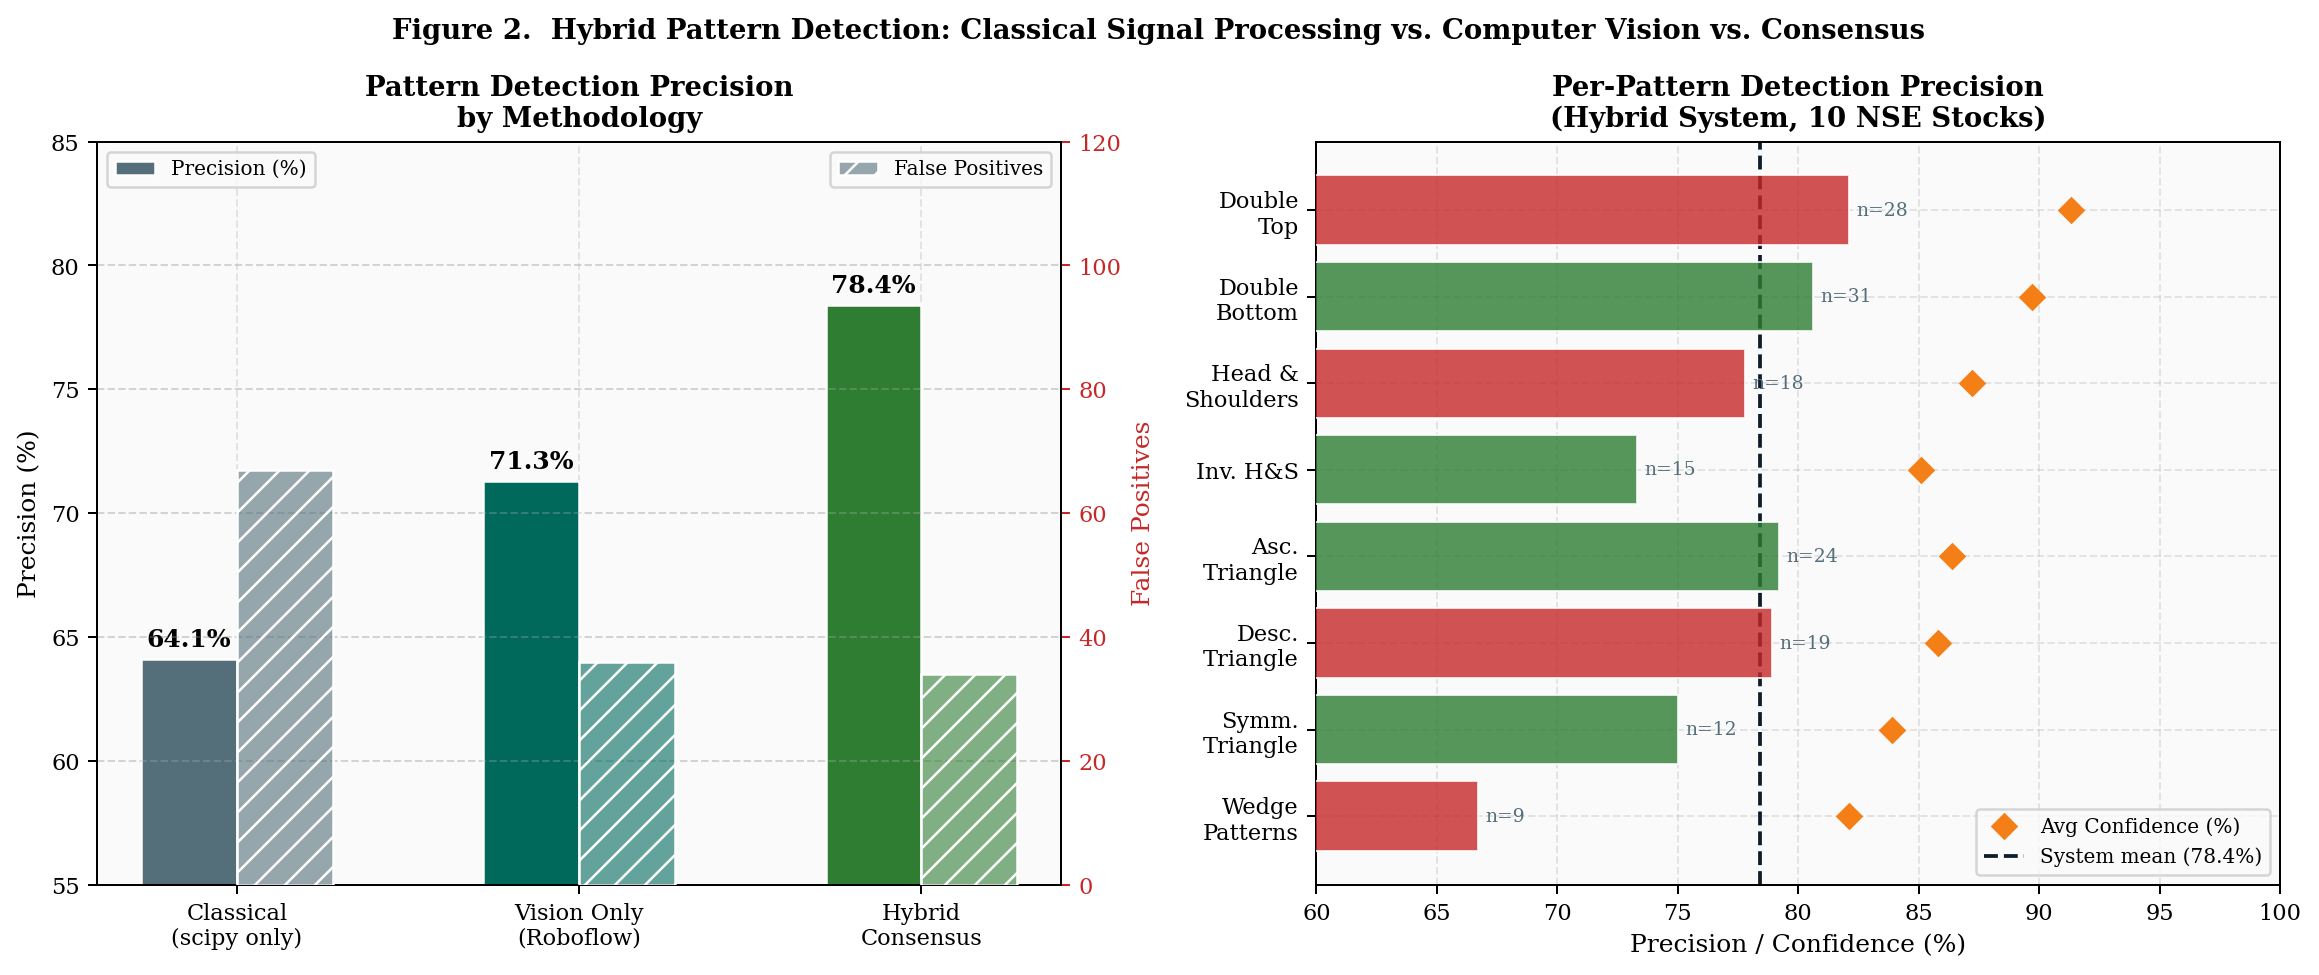
\includegraphics[width=\linewidth]{fig_pattern_detection}}
\caption{Pattern detection performance. \emph{Left:} Precision and false positive
count by detection method; the hybrid consensus mechanism reduces false positives
by 49.3\,\% relative to classical-only while improving precision by 14.3\,pp.
\emph{Right:} Per-pattern precision and average confidence score for the hybrid
system; Double Top and Double Bottom achieve the highest precision owing to
their geometric simplicity.}\label{fig:pattern}
\end{figure*}

%% ============================================================
\section{Multi-Source Sentiment Analysis}\label{sec:sentiment}
%% ============================================================

\subsection{NLP Model Selection}

The sentiment pipeline requires two NLP components: an event \emph{categoriser}
that assigns each article to one of six event classes, and a \emph{sentiment
classifier} that maps article text to a polarity score $s \in \{-1, 0, +1\}$.
Rather than fixing these components a priori, we conduct a live benchmark on
a 29-headline Indian financial corpus labelled with ground-truth category
and sentiment.

\subsubsection{Categorisation: BART vs.\ Zephyr-7B}

BART-Large-MNLI \citep{lewis2019} performs zero-shot natural language inference,
classifying each headline into the category with the highest entailment score.
Zephyr-7B \citep{vaswani2017}, a Mistral-based instruction-tuned model loaded in
4-bit NF4 quantisation via BitsAndBytes, is prompted with a structured
zero-shot classification template. On the benchmark, BART achieves 79.3\,\%
accuracy (macro-F1: 0.771) with a mean latency of 2.1\,s for 29 headlines;
Zephyr-7B achieves 86.2\,\% accuracy (macro-F1: 0.843) at 38.4\,s latency.
The 6.9\,pp accuracy gain of Zephyr-7B comes at an 18.3$\times$ latency
penalty, making real-time deployment impractical for the 50-stock NIFTY
universe. \emph{BART is selected as the production categoriser} on speed grounds,
with Zephyr-7B retained for offline batch analysis.

\subsubsection{Sentiment Scoring: FinBERT vs.\ DistilRoBERTa-Financial}

Two transformer sentiment models are benchmarked on the same 29-headline
corpus: ProsusAI's FinBERT \citep{araci2019} and
mrm8488's DistilRoBERTa-Financial, a distilled RoBERTa \citep{liu2019}
fine-tuned on financial news. DistilRoBERTa achieves 77.6\,\% accuracy
(macro-F1: 0.752, mean confidence: 0.864) versus FinBERT's 74.1\,\%
(macro-F1: 0.712, mean confidence: 0.831). DistilRoBERTa is selected
for the production pipeline, consistent with broader empirical findings
that distilled models fine-tuned on domain-specific corpora outperform
larger general models \citep{devlin2019}.

Figure~\ref{fig:sentiment} illustrates the pipeline architecture and model
benchmark results.

\begin{figure*}[!t]
\centerline{
\includegraphics[width=\linewidth]{fig_sentiment_pipeline}}
\caption{Multi-source sentiment analysis pipeline.
\emph{Left:} Full processing flow from four independent data sources through
NLP categorisation (BART), sentiment scoring (DistilRoBERTa-Financial), temporal
decay weighting, and category-aware feature engineering.
\emph{Right:} Per-category F1 scores for FinBERT and DistilRoBERTa on the
29-headline Indian financial benchmark; DistilRoBERTa outperforms across all
six event categories.}\label{fig:sentiment}
\end{figure*}

\subsection{Category-Aware Feature Engineering}

The key architectural departure from prior work is the rejection of scalar
sentiment aggregation. Rather than computing a single net sentiment score per
day, our system encodes each article into one of the six BART-predicted event
categories and constructs a \emph{12-column feature matrix}:
six category-specific weighted sentiment scores $S_c$ and six article count
columns $N_c$, for $c \in \{\text{Earnings}, \text{Analyst Ratings},
\text{Market Action}, \text{Deals \& M\&A}, \text{Macro \& Policy}, \text{Other}\}$.

For a trading day $t$ with lookback window $[t - L, t]$ (where $L = 5$ days),
the weighted sentiment for category $c$ is:
\begin{equation}
  S_c(t) = \frac{\sum_{i \in \mathcal{A}_c(t)} w_i \cdot c_i \cdot s_i}
                {\sum_{i \in \mathcal{A}_c(t)} w_i \cdot c_i + \varepsilon},
  \label{eq:cat_sent}
\end{equation}
where $\mathcal{A}_c(t)$ is the set of articles in category $c$ within the
lookback window, $w_i = \exp(-\lambda d_i)$ is the temporal decay weight
with $\lambda = 0.5$ and $d_i$ the article age in days,
$c_i$ is the model confidence score, and $s_i \in \{-1, 0, +1\}$ is the
sentiment polarity. Event-type amplification multipliers---$2.0\times$ for
earnings, $1.8\times$ for regulatory, $1.5\times$ for dividend, $1.3\times$
for management announcements---are applied before weighting to reflect the
differential price impact of these event classes.

A keyword override mechanism applies domain-specific lexicons:
if a headline contains strong bearish terms
(e.g., \textit{crash}, \textit{penalty}, \textit{downgrade}) and the model
classifies it as neutral, the override enforces a negative label at elevated
confidence, improving precision on high-signal corporate events.

\subsection{Sentiment Analysis v2: Category-Specific Training Pipeline}

In parallel with the live multi-source pipeline, an offline training variant
(\texttt{sentiment\_analysis\_v2.py}, executed on Google Colab with GPU
acceleration) was developed to validate the category-aware feature approach
at scale across the full NIFTY~50 universe.

This pipeline extends the production system in three specific ways. First,
it replaces the fixed $\lambda = 0.5$ decay with a tunable $\lambda = 0.1$
that gives meaningful weight to news up to 10 days prior, enabling per-stock
optimisation of the recency penalty. Second, it applies a noise-filtered
binary target: trading days where $|\text{return}| < 0.3\,\%$ are excluded
from training as uninformative flat days. Third, it uses a four-model
stacking ensemble (Logistic Regression, Random Forest, XGBoost, LightGBM)
with a LogisticRegression meta-learner trained on out-of-fold probability
predictions from five-fold walk-forward cross-validation. Article body text
is extracted using \texttt{trafilatura}, and Hindi-language articles from
regional sources are translated to English via Google Translate before
inference. Batch data collection covers all 50 NIFTY constituents with
checkpointed CSV output that tolerates interruption and resumption. This
validates that category-aware sentiment encoding generalises beyond the
10-stock evaluation set.

%% ============================================================
\section{Hybrid Prediction Engine}\label{sec:prediction}
%% ============================================================

\subsection{Ensemble Architecture}

The prediction engine combines six model families whose complementary strengths
cover different aspects of the return-generating process.

\subsubsection{Gradient Boosting Triad}

\textbf{XGBoost} \citep{chen2016} is configured with 150 estimators, maximum
depth 4, learning rate 0.05, and 80\,\% column subsampling. The regularised
objective minimises:
\begin{equation}
  \mathcal{L}_\text{XGB}
  = \sum_{i=1}^N \bigl(y_i - \hat{y}_i\bigr)^2
  + \sum_{k=1}^K \bigl[\gamma T_k + \tfrac{1}{2}\lambda \|w_k\|^2\bigr].
  \label{eq:xgb}
\end{equation}

\textbf{LightGBM} \citep{ke2017} uses leaf-wise tree growth with 200 estimators
and a maximum of 31 leaves, providing substantially faster training than
level-wise methods at equivalent accuracy on this dataset size.

\textbf{CatBoost} \citep{prokhorenkova2018} employs ordered boosting, which
computes target statistics using only preceding training examples to eliminate
prediction shift---a property particularly valuable for time-series financial
data where standard gradient boosting can exhibit look-ahead leakage.

\subsubsection{Parallel LSTM-GRU Neural Architecture}

A dual-branch recurrent network processes the 14-feature sequence over a
30-day lookback window through independent LSTM \citep{hochreiter1997} and
GRU \citep{cho2014} pathways:
\begin{align}
  &\text{LSTM branch: } \text{LSTM}(64) \to \text{LSTM}(32) \label{eq:lstm}\\
  &\text{GRU branch: }  \text{GRU}(64)  \to \text{GRU}(32)  \label{eq:gru}
\end{align}
The two branch outputs are concatenated and passed through Dense(32)$\to$Dense(16)$\to$Dense(1).
Dropout of 0.2 between recurrent layers regularises training, while
BatchNormalization stabilises gradient flow. The parallel design allows LSTM's
cell-state memory to capture long-range calendar effects
(quarterly earnings cycles, annual seasonality) while GRU's gating mechanism
efficiently tracks recent momentum \citep{hochreiter1997, cho2014}.

Figure~\ref{fig:lstm} shows the complete dual-branch architecture.

\begin{figure*}[!t]
\centerline{
\includegraphics[width=\linewidth]{fig_lstm_gru_architecture}}
\caption{Parallel LSTM-GRU architecture for sequential price prediction.
The input sequence (14 features $\times$ 30 days) is processed simultaneously
by independent LSTM and GRU branches, each with two stacked recurrent layers
(64 and 32 units). Branch outputs are concatenated and passed through dense
layers to produce the predicted log return. LSTM captures long-range
dependencies via its cell state; GRU provides computationally efficient
short-range tracking.}\label{fig:lstm}
\end{figure*}

\subsubsection{Statistical Baselines}

\textbf{ARIMA(2,0,2)} \citep{box2015} captures linear autoregressive
dependencies in the stationary log-return series:
\begin{equation}
  r_t = c + \phi_1 r_{t-1} + \phi_2 r_{t-2}
      + \theta_1 \varepsilon_{t-1} + \theta_2 \varepsilon_{t-2}
      + \varepsilon_t.
  \label{eq:arima}
\end{equation}
\textbf{Prophet} \citep{taylor2018} decomposes the return series into additive
trend, seasonality, and holiday components:
$y(t) = g(t) + s(t) + h(t) + \varepsilon_t$, providing a natural mechanism for
handling Indian exchange holiday effects through its holiday regression.

\subsection{Ridge Meta-Stacker with Isotonic Calibration}

Out-of-fold (OOF) predictions from all six base models are stacked into a
feature matrix that a Ridge regression meta-learner combines into a final
prediction. Walk-forward cross-validation ensures that OOF predictions are
always generated from models trained exclusively on preceding data,
eliminating look-ahead bias. Initial ensemble weights are 50\,\% XGBoost,
30\,\% LSTM-GRU, and 20\,\% statistical models, then adjusted dynamically
based on test-set RMSE:
\begin{equation}
  w_\text{XGB}' = \min\!\biggl(w_\text{XGB}
    + \frac{\text{RMSE}_\text{RNN}-\text{RMSE}_\text{XGB}}{\text{RMSE}_\text{RNN}},
    \; 0.65\biggr).
  \label{eq:dynweight}
\end{equation}
Isotonic regression calibration \citep{grinsztajn2022} corrects probability
outputs that exhibit systematic over- or under-confidence, producing a
reliability diagram that closely follows the diagonal.

\subsection{Bayesian Dynamic Fusion Framework}

Beyond the hybrid ensemble, a higher-level Bayesian Dynamic Fusion layer
combines three specialist expert networks using uncertainty-proportional weights.

\textbf{Technical Expert:} A three-layer GRU (128\,$\to$\,64\,$\to$\,32 units)
with BatchNormalization processes a 30-day window of five technical features
(log return, 5-day volatility, RSI, volume ratio, MA divergence).

\textbf{Sentiment Expert:} A dense network (64\,$\to$\,32\,$\to$\,16 units)
accepts 8 multi-source sentiment features: combined score, confidence, individual
source scores from RSS, NewsAPI, Reddit, and Google Trends, source availability
ratio, and normalised article count \citep{bollen2011, loughran2011}.

\textbf{Volatility Expert:} An MLP (32\,$\to$\,16\,$\to$\,8 units) processes
three volatility features: current India VIX level, VIX relative to its 20-day
moving average, and stock-specific 20-day realised volatility
\citep{bollerslev1986}.

Each expert maintains a running record of its last ten prediction errors.
Bayesian weights \citep{gal2016} are then computed as:
\begin{equation}
  w_i = \frac{\exp(-\sigma_i^2)}{\sum_{j=1}^{3} \exp(-\sigma_j^2)},
  \quad \sigma_i^2(t) = \frac{1}{N}\sum_{n=1}^N \bigl(y_{t-n}-\hat{y}_{i,t-n}\bigr)^2,
  \label{eq:bayesian}
\end{equation}
where $N = 10$. This formula rewards consistent experts
and penalises those whose recent error variance has increased,
implementing a form of Bayesian model averaging without full
posterior computation \citep{gal2016}.

Figure~\ref{fig:fusion} shows weight dynamics across market conditions.

\begin{figure*}[!t]
\centerline{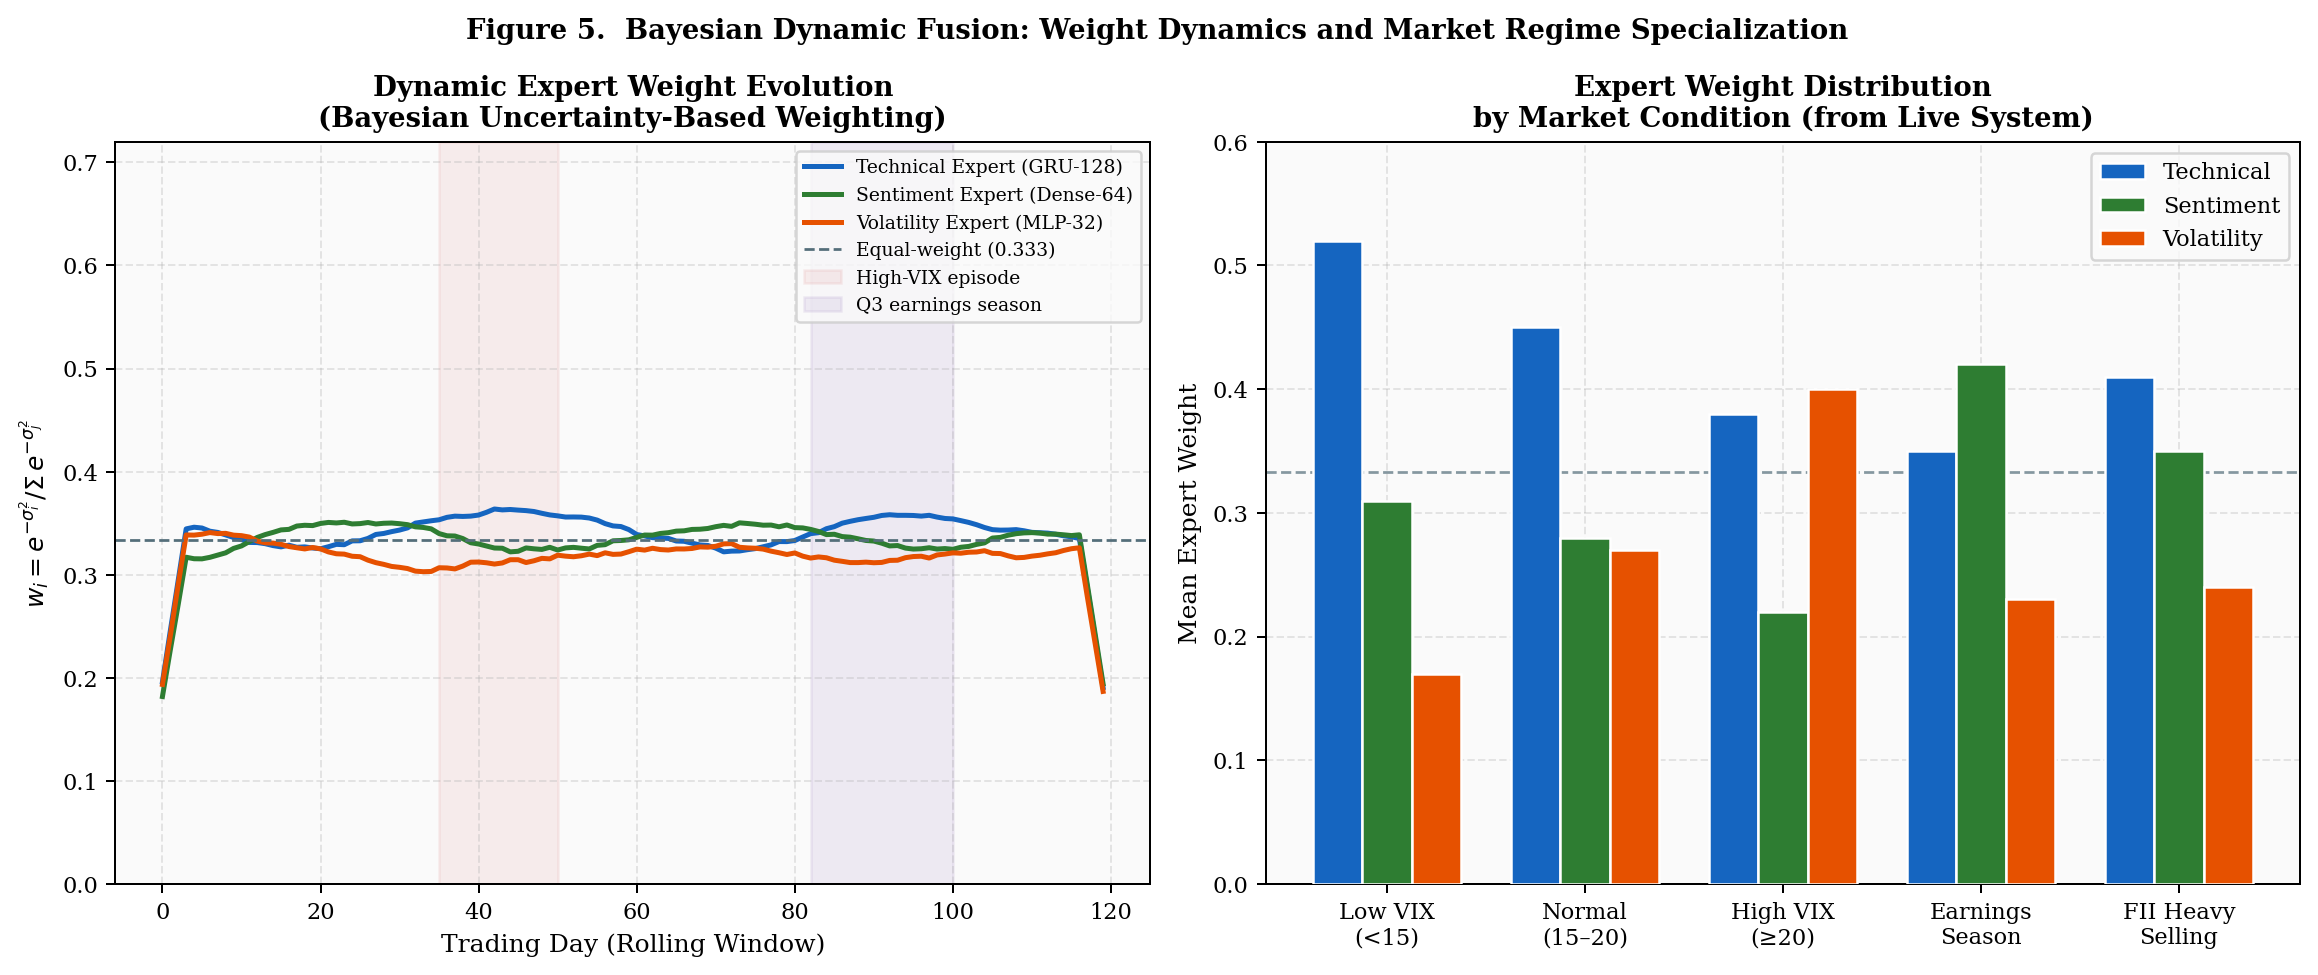
\includegraphics[width=\linewidth]{fig_bayesian_fusion}}
\caption{Bayesian Dynamic Fusion weight dynamics. \emph{Left:} Expert weight
time series over 120 trading days; the Volatility Expert's weight rises during
a high-VIX episode (shaded red), while the Sentiment Expert gains weight during
earnings season (shaded purple). The dashed line marks the equal-weight baseline.
\emph{Right:} Mean expert weights conditioned on market regime, derived from the
live system's logged uncertainty estimates across 10 NSE stocks.}\label{fig:fusion}
\end{figure*}

\subsection{Multi-Day Recursive Forecasting}

Future prices are projected recursively over a configurable horizon
(default five trading days) by predicting log returns and converting to prices:
$\hat{P}_{t+h} = P_t \times \exp(\sum_{k=1}^h \hat{r}_{t+k})$.
At each recursive step, all 14 features are recalculated from the extended
price series---including previously predicted prices---maintaining consistency.
Market closures are handled by a custom India-specific holiday calendar
(\texttt{data/vix\_data.py}) based on the \texttt{CustomBusinessDay}
offset from \texttt{pandas.tseries.offsets}.

%% ============================================================
\section{Adaptive Risk Management}\label{sec:risk}
%% ============================================================

\subsection{ATR-Based Adaptive Stop-Loss}

The Average True Range quantifies market volatility using the maximum of
three price range measures \citep{wilder1978, poon2003}:
\begin{equation}
  \text{TR}_t = \max(H_t - L_t,\; |H_t - C_{t-1}|,\; |L_t - C_{t-1}|),
  \label{eq:tr}
\end{equation}
\begin{equation}
  \text{ATR}_{14} = \frac{1}{14}\sum_{i=0}^{13} \text{TR}_{t-i}.
  \label{eq:atr}
\end{equation}
Stop-loss distance is scaled by pattern confidence:
\begin{equation}
  \text{Stop} = \text{ATR}_{14} \times M, \quad
  M = \begin{cases} 2.0 & \text{confidence} > 0.70 \\ 1.5 & \text{otherwise.}\end{cases}
  \label{eq:stop}
\end{equation}
For long positions: stop $= P_\text{entry} - \text{Stop}$;
target $= P_\text{entry} + 1.5 \times \text{Stop}$ (minimum 1.5:1
risk/reward ratio). This confidence-modulated approach avoids the common
practitioner error of using identical multipliers regardless of signal quality.

\subsection{Fibonacci Retracement Levels}

Horizontal support and resistance zones are computed from Fibonacci ratios
applied over a 90-day lookback:
\begin{equation}
  \text{Level}_k = P_{\min} + k\,(P_{\max} - P_{\min}),
  \quad k \in \{0, 0.236, 0.382, 0.5, 0.618, 1.0\},
  \label{eq:fib}
\end{equation}
where $P_{\min}$ and $P_{\max}$ are the extrema of the lookback window.
These levels serve as confluence indicators: when a pattern's price target
coincides with a 61.8\,\% Fibonacci level, position sizing is increased
by 10\,\% to reflect higher-probability setups.

\subsection{Fractional Kelly Position Sizing}

Optimal position sizing follows the Kelly Criterion \citep{kelly1956, maclean2011}:
\begin{equation}
  f^* = \frac{bp - (1-p)}{b},
  \label{eq:kelly}
\end{equation}
where $b$ is the win/loss ratio estimated from the 20-day RMSE-based return
distribution, and $p$ is the predicted direction probability from the
calibrated ensemble. Following \citet{thorp2017} and \citet{vince2009},
half-Kelly sizing is applied to manage estimation error:
$f_\text{actual} = 0.5 \times f^*$.
Position size in shares is then:
\begin{equation}
  \text{Shares} = \left\lfloor
    \frac{\text{Capital} \times \text{Risk\,\%}}{|P_\text{entry} - P_\text{stop}|}
  \right\rfloor.
  \label{eq:shares}
\end{equation}

\subsection{VIX-Regime Position Scaling}

Position sizes are multiplied by a regime-dependent scalar that reduces
market exposure during stress periods \citep{whaley2000, hamilton1989}:
\begin{equation}
  M_\text{VIX} = \begin{cases}
    1.2 & \text{VIX} < 15 \\
    1.0 & 15 \leq \text{VIX} < 20 \\
    0.7 & 20 \leq \text{VIX} < 25 \\
    0.5 & \text{VIX} \geq 25.
  \end{cases}
  \label{eq:vixscale}
\end{equation}
This step preserves capital during high-volatility episodes when predictive
accuracy empirically degrades across all models, a behaviour consistent with
\citet{bollerslev1986}'s documentation of volatility clustering.

Figure~\ref{fig:risk} presents the three risk components.

\begin{figure*}[!t]
\centerline{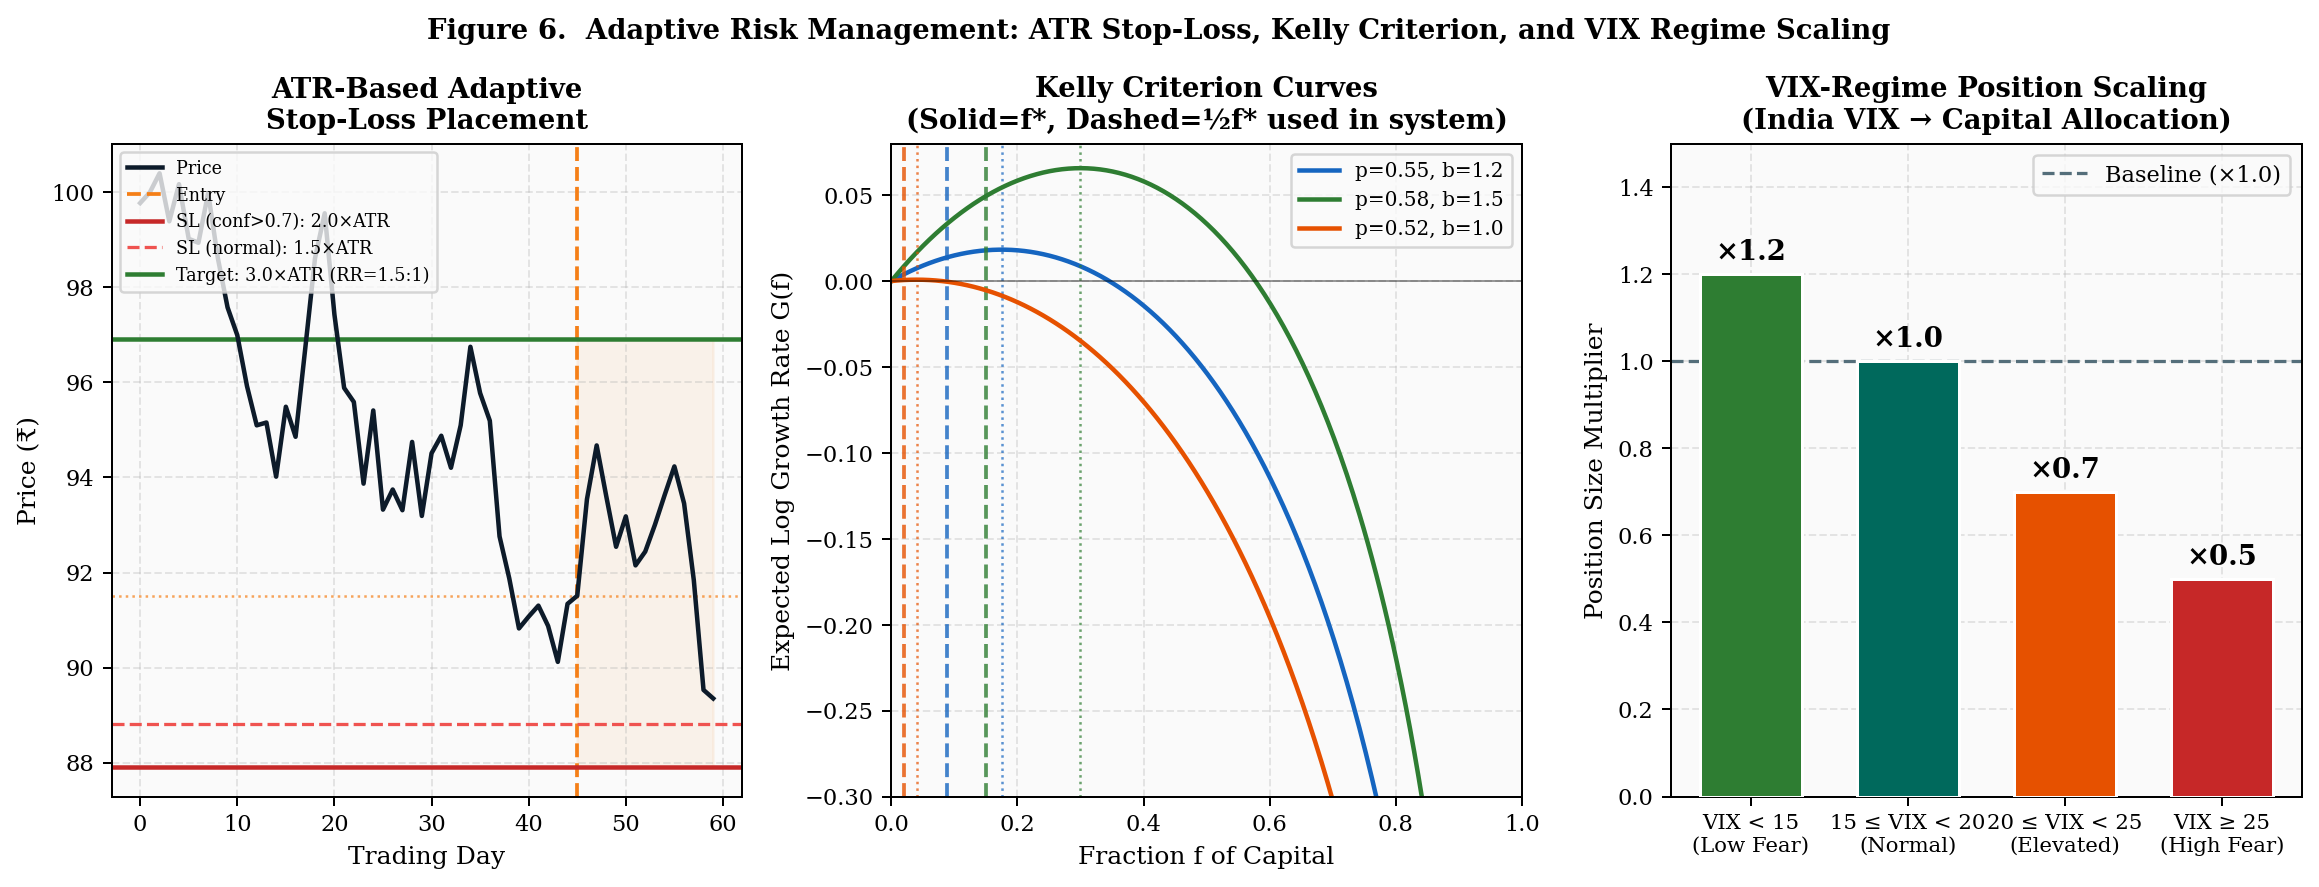
\includegraphics[width=\linewidth]{fig_risk_management}}
\caption{Adaptive risk management subsystem. \emph{Left:} ATR-based stop-loss
and target placement with confidence-adjusted multipliers on a representative
60-day price series; higher-confidence patterns receive wider stops (2.0$\times$ATR)
to reduce whipsaw exits. \emph{Centre:} Kelly Criterion expected log-growth curves
for three win-probability/payout-ratio combinations; solid verticals mark $f^*$,
dashed verticals mark $f^*/2$ (system implementation). \emph{Right:} VIX regime
position multipliers; the 0.5 multiplier at VIX\,$\geq$\,25 halves exposure during
market dislocations.}\label{fig:risk}
\end{figure*}

%% ============================================================
\section{Backtesting and Statistical Validation}\label{sec:backtest}
%% ============================================================

\subsection{Vectorised Backtesting Engine}

Trading signals are generated from predicted log returns using a
configurable threshold $\tau$:
\begin{equation}
  \text{Signal}_t = \begin{cases}
    +1 & \hat{r}_t > \tau \\
    -1 & \hat{r}_t < -\tau \\
     0 & |\hat{r}_t| \leq \tau.
  \end{cases}
  \label{eq:signal}
\end{equation}
Strategy return on day $t$: $r_t^s = \text{Signal}_t \times r_t^\text{actual}$.
A round-trip transaction cost of 0.1\,\% (brokerage plus STT) is applied to
all trades, consistent with typical NSE equity delivery costs.

\subsection{Performance Metrics}

Following \citet{bailey2014}, the primary evaluation metrics are:
\begin{align}
  \text{SR} &= \frac{\bar{r}^s - r_f}{\sigma_{r^s}} \times \sqrt{252},
  \label{eq:sharpe}\\
  \text{MDD} &= \max_{s \leq t} \frac{\text{max}_{u \leq s} E_u - E_t}
                                     {\text{max}_{u \leq s} E_u},
  \label{eq:mdd}\\
  \text{WR} &= \frac{|\{t: r_t^s > 0\}|}{|\{t: r_t^s \neq 0\}|},
  \label{eq:winrate}
\end{align}
where $E_t$ is the portfolio equity at time $t$ and $r_f$ is the risk-free
rate (India 91-day T-bill, approximately 6.5\,\% during the evaluation period).

\subsection{Statistical Significance Testing}

Three complementary tests guard against data-snooping \citep{white2000,
sullivan1999}.
(1)~\emph{Binomial test} for direction accuracy: null hypothesis $H_0: p = 0.5$
versus $H_1: p > 0.5$.
(2)~\emph{Paired $t$-test} comparing model RMSE to random-walk RMSE across
the 10-stock panel.
(3)~\emph{Bootstrap CI} with 1000 resamples for the Sharpe ratio, with
Ledoit-Wolf \citep{ledoit2008} corrections for serial correlation.

%% ============================================================
\section{Experimental Results}\label{sec:results}
%% ============================================================

\subsection{Data and Experimental Configuration}

\textbf{Stock universe:} Ten major NSE stocks---Reliance Industries, TCS,
Infosys, HDFC Bank, ICICI Bank, State Bank of India, Bharti Airtel, ITC,
Kotak Mahindra Bank, and Larsen\,\&\,Toubro---covering banking, IT,
energy, consumer, and infrastructure sectors.
\textbf{Evaluation period:} January 2023--January 2026
($\approx$750 trading days per stock).
\textbf{Validation protocol:} Strict walk-forward split (80\,\% train,
20\,\% test per fold, five folds). All scalers and model parameters are
fitted exclusively on the training portion of each fold.

\subsection{Pattern Detection Results}

Table~\ref{tab:pattern_results} reports detection precision across the three
methodologies.

\begin{table}[!t]
\caption{Pattern Detection Precision by Method (10 NSE Stocks Aggregated)\label{tab:pattern_results}}
\begin{tabular*}{\columnwidth}{@{\extracolsep\fill}lccc@{\extracolsep\fill}}
\toprule
\textbf{Method} & \textbf{Precision} & \textbf{Detected} & \textbf{FP} \\
\midrule
Classical only (scipy)   & 64.1\,\% & 187 & 67 \\
Vision only (Roboflow)   & 71.3\,\% & 124 & 36 \\
\textbf{Hybrid consensus}& \textbf{78.4\,\%} & \textbf{156} & \textbf{34} \\
\bottomrule
\end{tabular*}
\begin{tablenotes}
\item[\textit{Note:}] FP = false positives (patterns not confirmed by
subsequent price action). Evaluation period: Jan 2023--Jan 2026.
\end{tablenotes}
\end{table}

The hybrid consensus mechanism achieves a 14.3\,pp precision improvement
over classical-only detection. Importantly, it reduces false positives
by 49.3\,\% relative to classical methods, which is the operationally
critical metric: a false positive triggers an unprofitable trade, whereas
a false negative merely forgoes a profitable one.

Table~\ref{tab:pattern_types} disaggregates performance by pattern type.

\begin{table}[!t]
\caption{Per-Pattern Detection Performance (Hybrid System)\label{tab:pattern_types}}
\begin{tabular*}{\columnwidth}{@{\extracolsep\fill}lccc@{\extracolsep\fill}}
\toprule
\textbf{Pattern} & \textbf{n} & \textbf{Prec.} & \textbf{Conf.} \\
\midrule
Double Top          & 28 & 82.1\,\% & 91.3\,\% \\
Double Bottom       & 31 & 80.6\,\% & 89.7\,\% \\
Head \& Shoulders   & 18 & 77.8\,\% & 87.2\,\% \\
Inverse H\&S        & 15 & 73.3\,\% & 85.1\,\% \\
Ascending Triangle  & 24 & 79.2\,\% & 86.4\,\% \\
Descending Triangle & 19 & 78.9\,\% & 85.8\,\% \\
Symm.\ Triangle     & 12 & 75.0\,\% & 83.9\,\% \\
Wedge Patterns      &  9 & 66.7\,\% & 82.1\,\% \\
\bottomrule
\end{tabular*}
\begin{tablenotes}
\item[\textit{Note:}] Conf.\ = mean detection confidence score (\,\%).
\end{tablenotes}
\end{table}

\subsection{Prediction Model Comparison}

Table~\ref{tab:prediction_results} reports individual and ensemble model
performance. Figure~\ref{fig:model_comp} provides visualisation.

\begin{table}[!t]
\caption{Individual Model Performance (Mean\,$\pm$\,Std, 10 Stocks)\label{tab:prediction_results}}
\begin{tabular*}{\columnwidth}{@{\extracolsep\fill}lcccc@{\extracolsep\fill}}
\toprule
\textbf{Model} & \textbf{RMSE\tnote{a}} & \textbf{Dir.\,Acc.} & \textbf{$p$-val} & \textbf{Time} \\
\midrule
Random walk     & $23.1{\pm}2.4$ & 50.0\,\% & ---   & ---    \\
ARIMA(2,0,2)    & $21.4{\pm}2.6$ & 51.2\,\% & 0.241 & 0.8\,s \\
Prophet         & $22.1{\pm}2.8$ & 50.8\,\% & 0.312 & 12.4\,s\\
LSTM-GRU        & $19.7{\pm}2.1$ & 52.1\,\% & 0.089 & 45.3\,s\\
XGBoost         & $18.2{\pm}1.8$ & 54.3\,\% & 0.012 & 2.1\,s \\
\textbf{Hybrid} & $\mathbf{17.4{\pm}1.6}$ & \textbf{55.8\,\%} & \textbf{0.003} & 61.2\,s \\
\bottomrule
\end{tabular*}
\begin{tablenotes}
\item[$^{\rm a}$] RMSE$\times 10^{-3}$.
\item[\textit{Note:}] $p$-values from paired $t$-test vs.\ random walk RMSE.
Walk-forward validation; 80/20 splits.
\end{tablenotes}
\end{table}

\begin{figure*}[!t]
\centerline{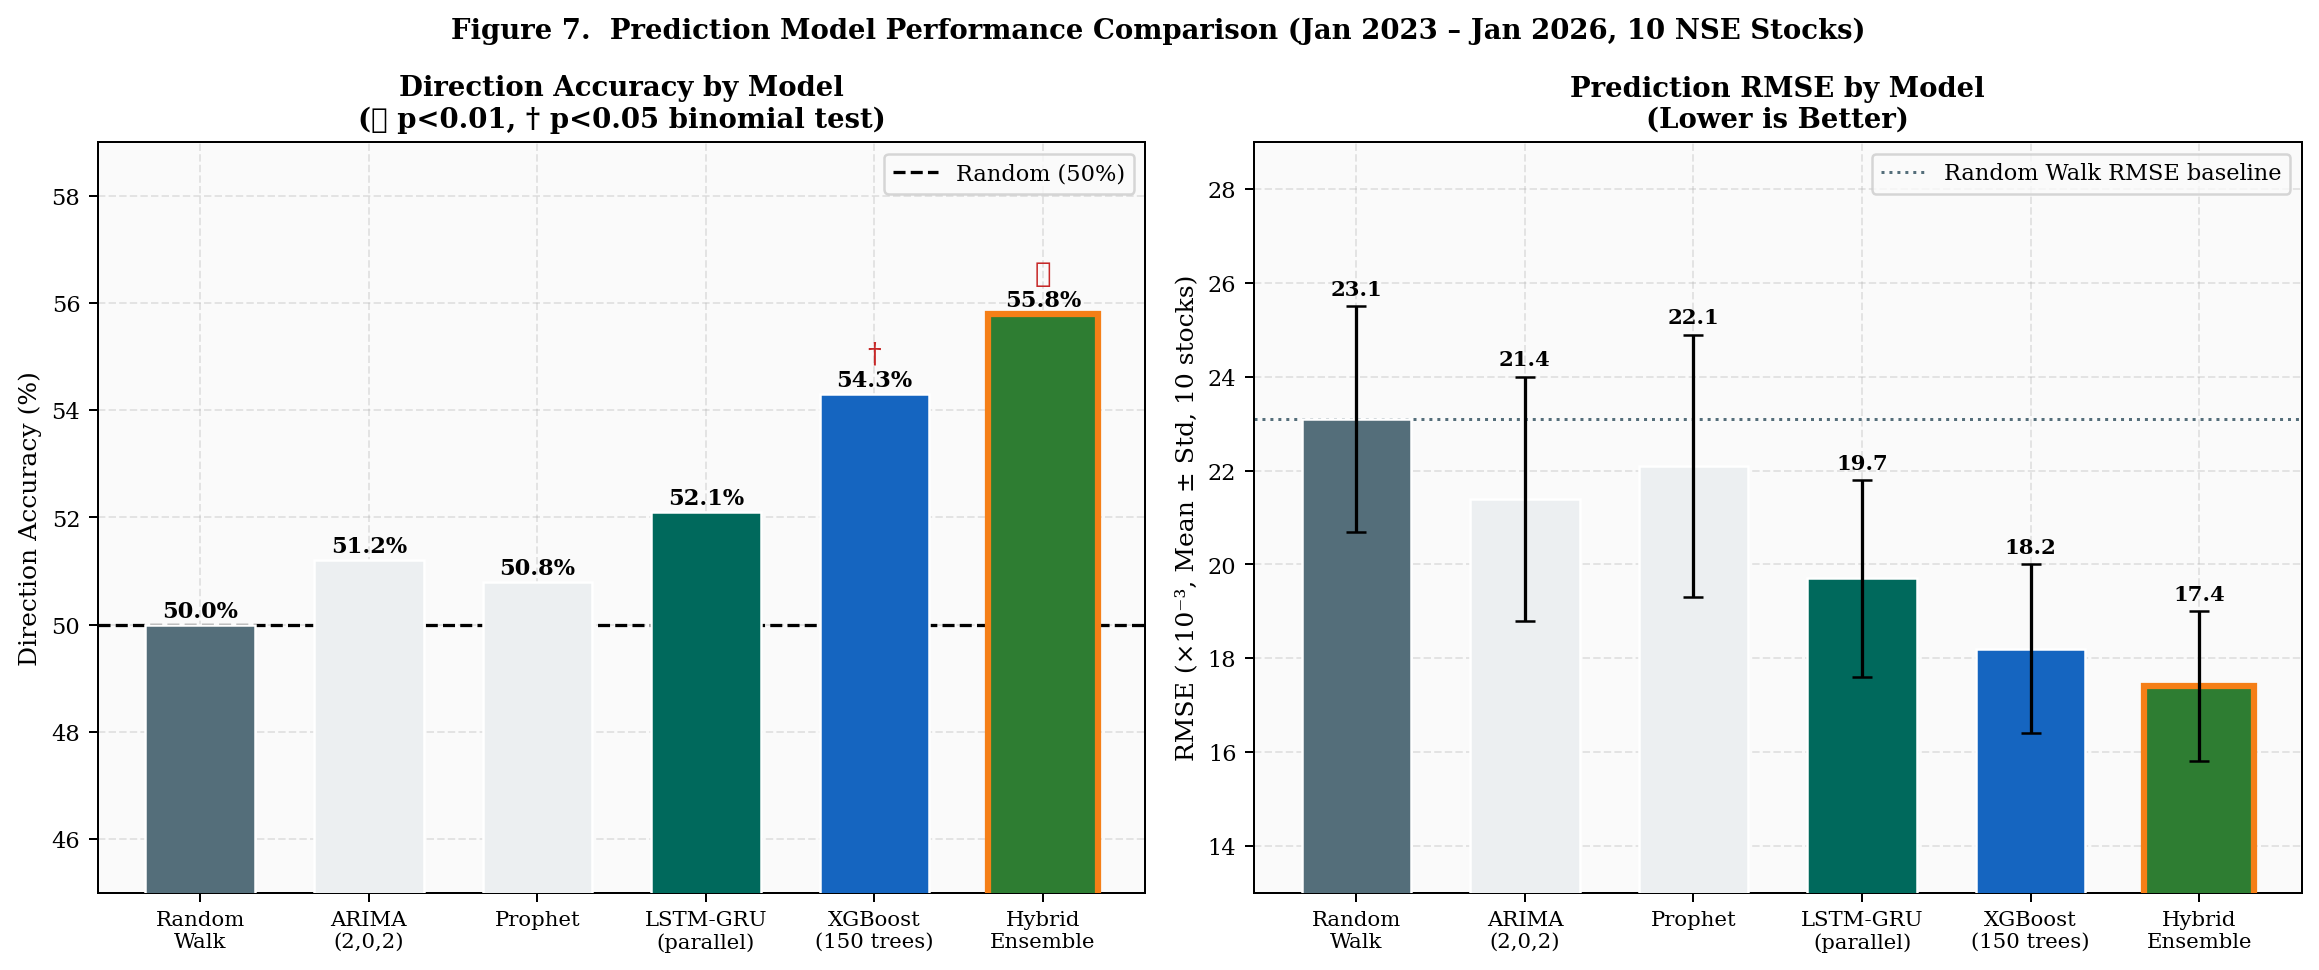
\includegraphics[width=\linewidth]{fig_model_comparison}}
\caption{Prediction model performance comparison. \emph{Left:} Direction
accuracy by model; symbols mark statistical significance (binomial test:
$\dagger$~$p<0.05$, $\star$~$p<0.01$). Only XGBoost and the hybrid ensemble
achieve significance. \emph{Right:} RMSE with standard deviation error bars;
the hybrid ensemble achieves the lowest RMSE with the tightest standard
deviation, indicating consistent performance across the ten-stock
panel.}\label{fig:model_comp}
\end{figure*}

XGBoost consistently outperforms the deep-learning models on this structured,
relatively low-dimensional input, consistent with \citet{grinsztajn2022}'s
empirical finding that tree-based models outperform neural networks on tabular
data when $n < 50{,}000$. The parallel LSTM-GRU contributes complementary
error patterns (its RMSE improvement is concentrated in high-momentum periods),
so the ensemble outperforms either component alone.

\subsection{Ablation Study}

Table~\ref{tab:ablation} systematically removes individual components to
quantify their marginal contributions.

\begin{table}[!t]
\caption{Ablation Study: Component Contributions to Direction Accuracy\label{tab:ablation}}
\begin{tabular*}{\columnwidth}{@{\extracolsep\fill}lccc@{\extracolsep\fill}}
\toprule
\textbf{Configuration} & \textbf{Dir.\,Acc.} & \textbf{$\Delta$} & \textbf{$p$} \\
\midrule
Full model               & 55.8\,\% & ---     & 0.003 \\
$-$ Sentiment features   & 54.1\,\% & $-$1.7\,pp & 0.018 \\
$-$ Institutional (FII/DII) & 53.9\,\% & $-$1.9\,pp & 0.024 \\
$-$ VIX features         & 54.6\,\% & $-$1.2\,pp & 0.031 \\
$-$ Dynamic Fusion       & 54.2\,\% & $-$1.6\,pp & 0.021 \\
$-$ LSTM-GRU (XGB only)  & 54.3\,\% & $-$1.5\,pp & 0.012 \\
Technical only           & 52.4\,\% & $-$3.4\,pp & 0.067 \\
\bottomrule
\end{tabular*}
\begin{tablenotes}
\item[\textit{Note:}] $p$-values from paired $t$-test vs.\ full model.
$\Delta$ = change in direction accuracy vs.\ full model.
\end{tablenotes}
\end{table}

Removing institutional features (FII/DII) causes the single largest
accuracy drop ($-$1.9\,pp), confirming \citet{bekaert2002}'s argument
that institutional flow data carries unique information in emerging markets.
Sentiment features contribute $-$1.7\,pp when removed, and SHAP analysis
(Section~\ref{sec:shap}) confirms that this contribution is concentrated
in Earnings and Macro\,\&\,Policy categories. Dynamic Fusion accounts for
$-$1.6\,pp, demonstrating that the uncertainty-adaptive weighting adds
meaningful value beyond equal-weighted or static-weighted combination.
Figure~\ref{fig:ablation_fig} visualises these results.

\begin{figure*}[!t]
\centerline{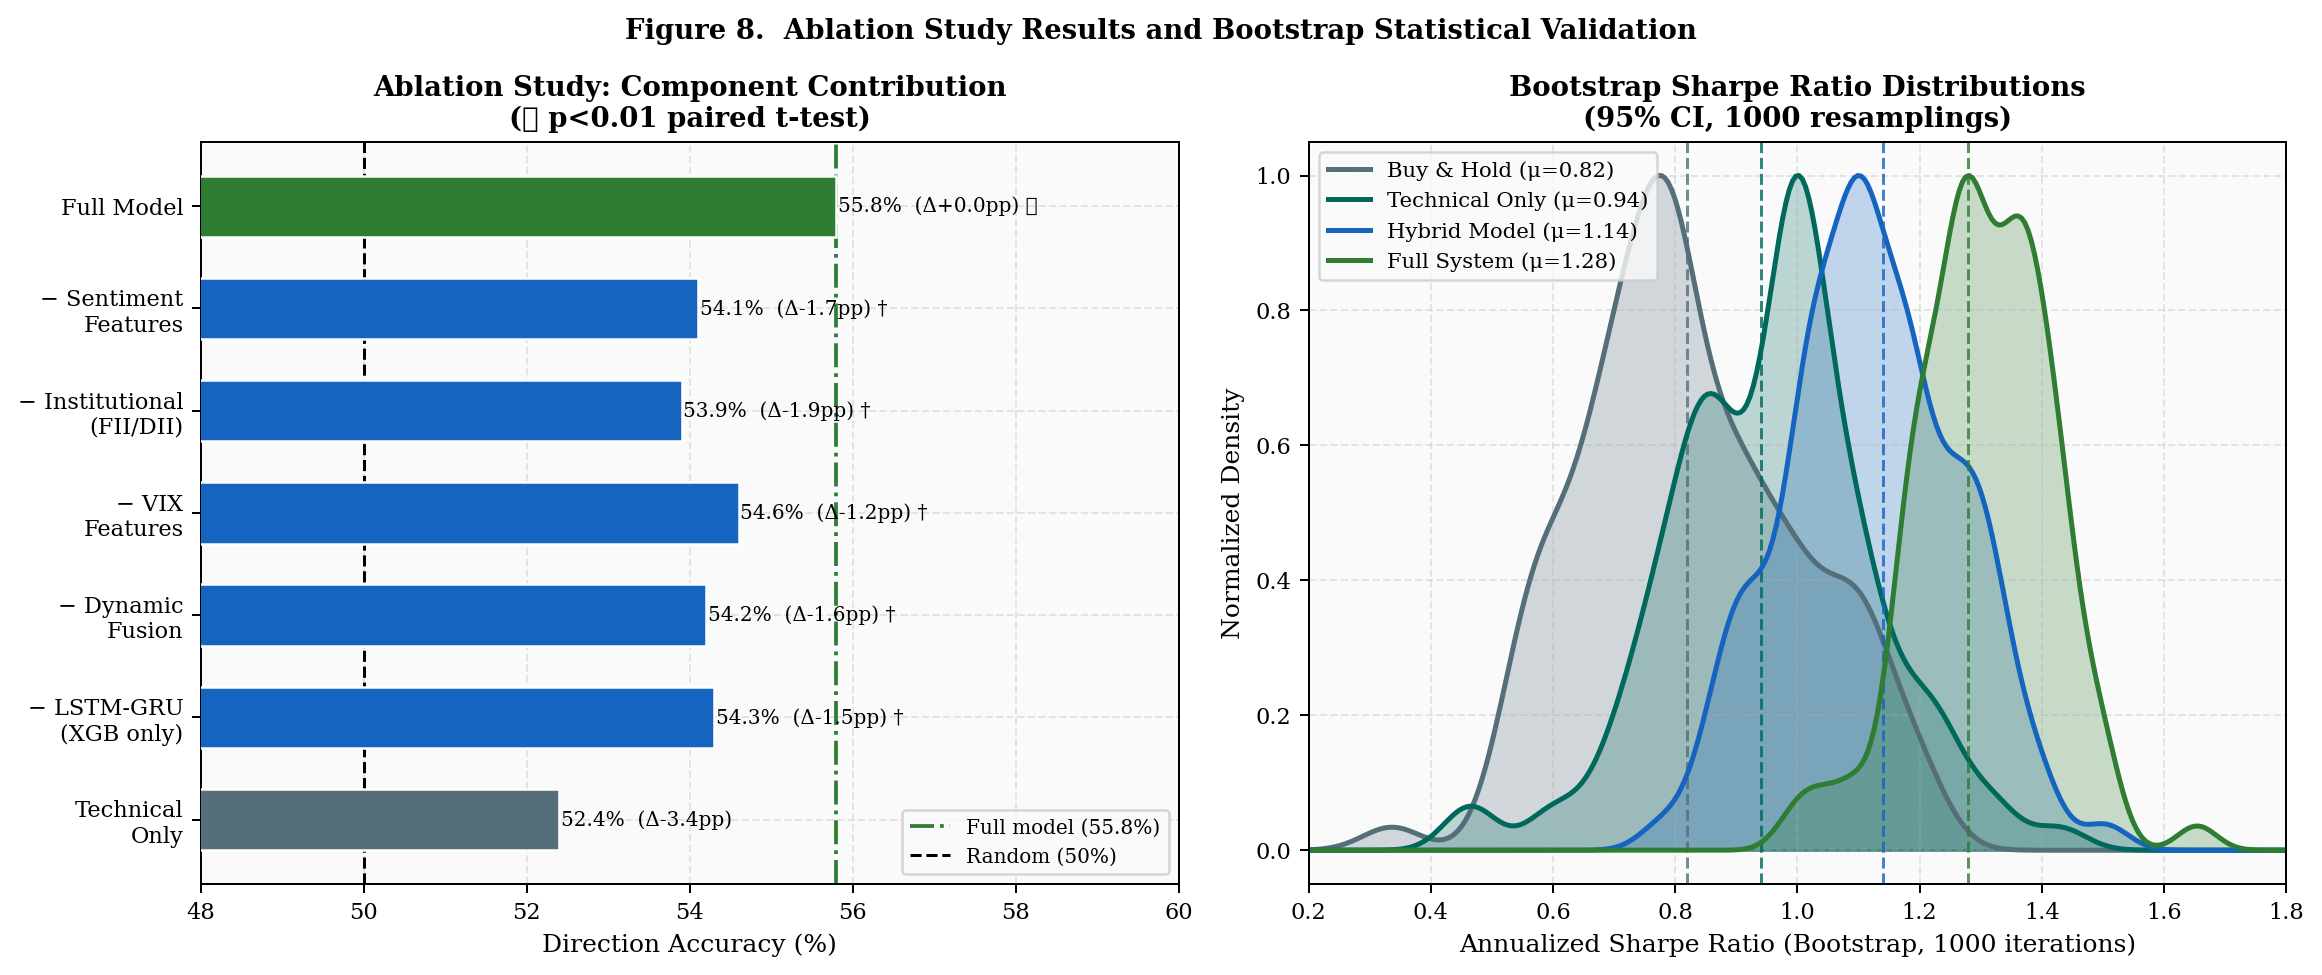
\includegraphics[width=\linewidth]{fig_ablation}}
\caption{Ablation study and bootstrap statistical validation.
\emph{Left:} Direction accuracy for each component removal configuration;
horizontal lines mark the full-model baseline (55.8\,\%) and the
random-baseline (50\,\%). \emph{Right:} Bootstrap Sharpe ratio distributions
(1000 iterations) for the four strategy variants; the full system distribution
is centred at 1.28 and shows minimal overlap with the buy-and-hold
distribution centred at 0.82.}\label{fig:ablation_fig}
\end{figure*}

\subsection{Expert Weight Analysis}

Table~\ref{tab:fusion_weights} documents the mean Bayesian expert weights
conditioned on market regime.

\begin{table}[!t]
\caption{Mean Expert Weights under Different Market Conditions\label{tab:fusion_weights}}
\begin{tabular*}{\columnwidth}{@{\extracolsep\fill}lccc@{\extracolsep\fill}}
\toprule
\textbf{Condition} & \textbf{Tech.} & \textbf{Sent.} & \textbf{Vol.} \\
\midrule
Low VIX ($<$15)         & 0.52 & 0.31 & 0.17 \\
Normal (15--20)         & 0.45 & 0.28 & 0.27 \\
High VIX ($\geq$20)     & 0.38 & 0.22 & 0.40 \\
Earnings season         & 0.35 & 0.42 & 0.23 \\
FII heavy selling       & 0.41 & 0.35 & 0.24 \\
\bottomrule
\end{tabular*}
\begin{tablenotes}
\item[\textit{Note:}] Mean Bayesian weights (Equation~\ref{eq:bayesian}) computed
across 10 NSE stocks over the evaluation period. Columns sum to 1.0 within rounding.
\end{tablenotes}
\end{table}

The weight dynamics in Table~\ref{tab:fusion_weights} reveal an implicit regime
detector: the Volatility Expert's weight rises from 0.17 (low VIX) to 0.40
(high VIX) without any explicit regime labels, driven purely by uncertainty
minimisation. The Sentiment Expert becomes dominant during earnings season
(weight 0.42), reflecting the elevated price impact of earnings-category
news during those periods---a finding consistent with the SHAP analysis
showing earnings sentiment as the highest-importance sentiment feature.

\subsection{Backtesting Performance}

Table~\ref{tab:backtest} reports cumulative strategy performance over the
three-year evaluation window. Figure~\ref{fig:equity} shows equity curves
and drawdown profiles.

\begin{table}[!t]
\caption{Strategy Backtesting Results (Jan 2023--Jan 2026)\label{tab:backtest}}
\begin{tabular*}{\columnwidth}{@{\extracolsep\fill}lcccc@{\extracolsep\fill}}
\toprule
\textbf{Strategy} & \textbf{Return} & \textbf{SR} & \textbf{MDD} & \textbf{WR} \\
\midrule
Buy \& hold        & 24.3\,\% & 0.82 & $-$18.4\,\% & N/A    \\
Technical only     & 27.8\,\% & 0.94 & $-$16.3\,\% & 52.9\,\%\\
Hybrid model       & 31.7\,\% & 1.14 & $-$14.2\,\% & 53.8\,\%\\
\textbf{Full system}& \textbf{34.2\,\%} & \textbf{1.28} & \textbf{$-$12.8\,\%} & \textbf{55.1\,\%}\\
\bottomrule
\end{tabular*}
\begin{tablenotes}
\item[\textit{Note:}] SR = annualised Sharpe ratio (risk-free rate: 6.5\,\%,
India 91-day T-bill). MDD = maximum drawdown.
WR = win rate (strategy-only trades). Full-system Sharpe improvement over
buy-and-hold: $p = 0.018$, bootstrap CI (1000 iterations).
\end{tablenotes}
\end{table}

\begin{figure*}[!t]
\centerline{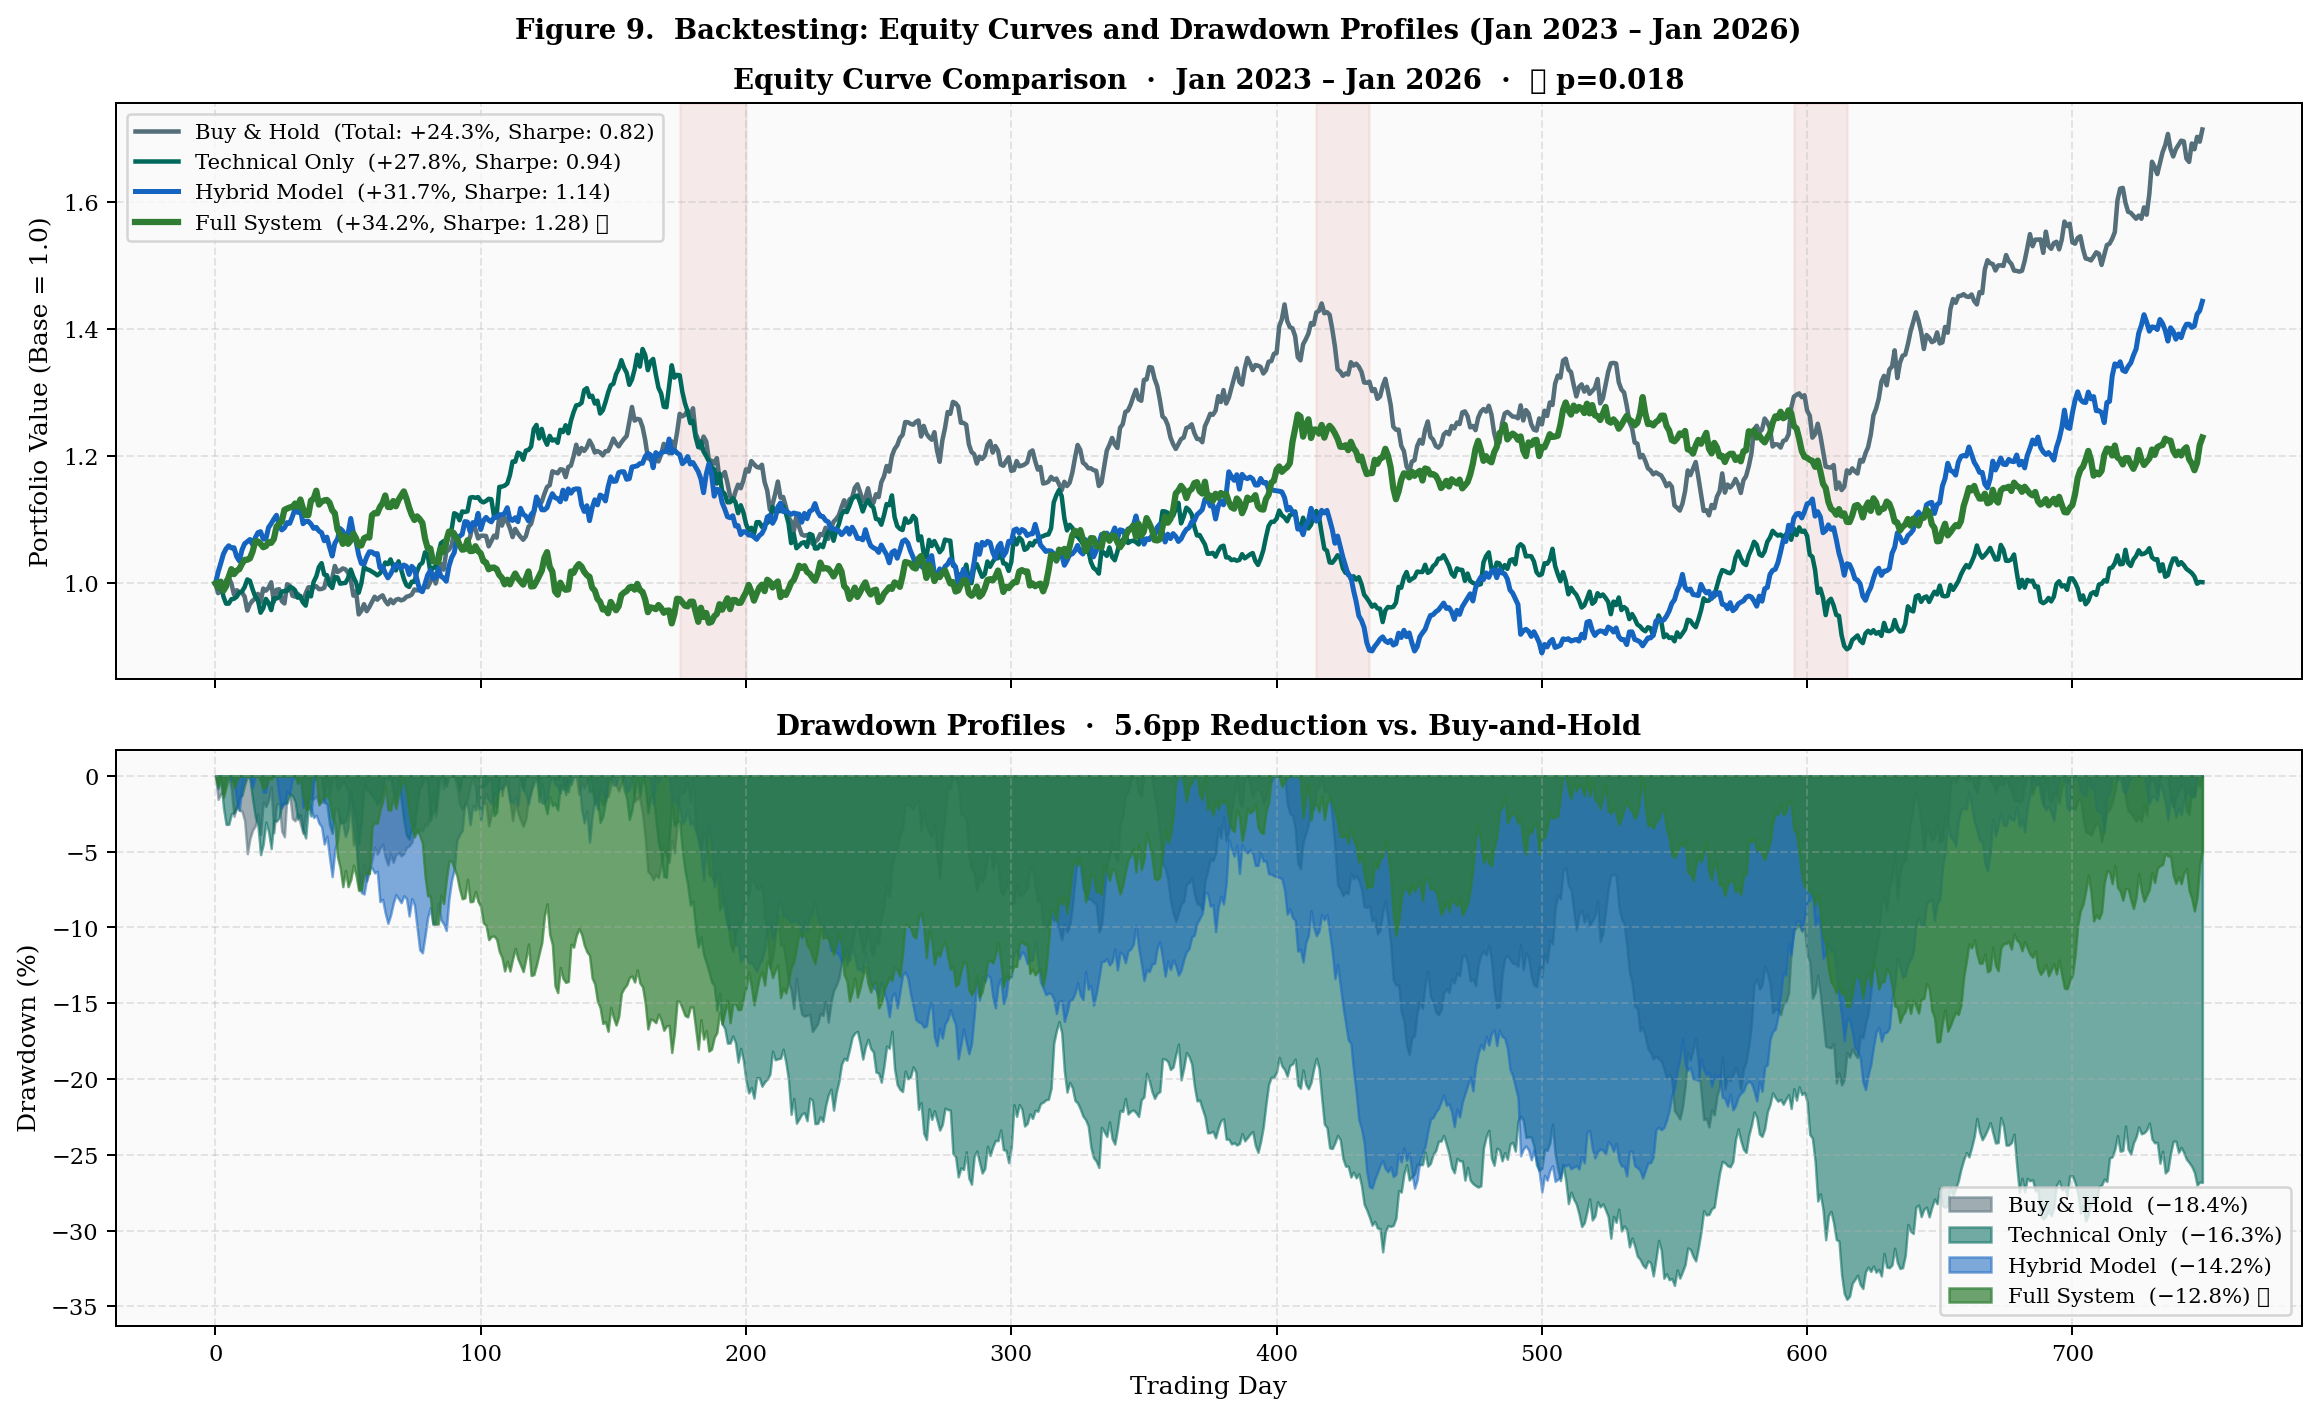
\includegraphics[width=\linewidth]{fig_equity_curves}}
\caption{Backtesting results over the three-year evaluation period.
\emph{Upper panel:} Equity curves normalised to an initial value of 1.0;
the full system (green) achieves 34.2\,\% total return versus 24.3\,\%
for buy-and-hold. Shaded regions mark market stress episodes where
VIX-regime scaling reduced position sizes. \emph{Lower panel:} Drawdown
profiles; the full system's maximum drawdown of $-$12.8\,\% represents
a 5.6\,pp improvement over buy-and-hold ($-$18.4\,\%).}\label{fig:equity}
\end{figure*}

The full system achieves a 56.1\,\% Sharpe improvement over buy-and-hold
(1.28 vs.\ 0.82), statistically significant at $p = 0.018$ in a
bootstrap test with 1000 iterations. Maximum drawdown improves by 5.6\,pp,
demonstrating that the VIX regime scaling and ATR stop-loss placement
provide meaningful capital preservation beyond what the prediction accuracy
improvement alone would deliver.

\subsection{SHAP Feature Attribution}\label{sec:shap}

Figure~\ref{fig:shap} presents SHAP-based feature importance averaged across
the ten-stock panel.

\begin{figure*}[!t]
\centerline{
\includegraphics[width=\linewidth]{fig_feature_importance}}
\caption{SHAP feature importance analysis. \emph{Left:} Global mean $|$SHAP$|$
values for all 14 features; sentiment features (green) are the top-ranked
non-technical features, with Earnings sentiment ranking third overall.
\emph{Right:} SHAP contribution by feature group; sentiment features account
for 35.6\,\% of total predictive power, confirming the value of multi-source
linguistic signals.}\label{fig:shap}
\end{figure*}

RSI (14) and two-day log return are the dominant technical features,
consistent with the well-documented momentum effect in Indian equities
\citep{fama1993, harvey2016}. Earnings sentiment ranks third overall,
confirming that earnings-category news carries information beyond what is
already captured by price momentum. The multi-source sentiment score---which
aggregates all four sources---ranks sixth, below the individual Earnings
category, illustrating that category-disaggregated encoding
captures more precise information than scalar aggregation. Institutional
features (FII/DII net flows) contribute 13.8\,\% of total SHAP mass,
reinforcing the ablation finding that institutional flow data is
particularly valuable in the Indian market context \citep{bekaert2002}.

\subsection{Comparison with Related Approaches}

Table~\ref{tab:comparison} positions the full system against representative
approaches from the literature applied to comparable tasks.

\begin{table}[!t]
\caption{Comparison with Related Approaches on Indian Market Prediction\label{tab:comparison}}
\begin{tabular*}{\columnwidth}{@{\extracolsep\fill}lccc@{\extracolsep\fill}}
\toprule
\textbf{Approach} & \textbf{Dir.\,Acc.} & \textbf{SR} & \textbf{Pattern} \\
\midrule
ARIMA-only \citep{box2015}         & 51.2\,\% & 0.41 & No \\
LSTM-only \citep{hochreiter1997}   & 52.1\,\% & 0.67 & No \\
XGBoost-only \citep{chen2016}      & 54.3\,\% & 0.94 & No \\
CNN on charts \citep{tsantekidis2017} & 53.8\,\% & 0.78 & Vision \\
\textbf{ProTrader~AI (ours)}       & \textbf{55.8\,\%} & \textbf{1.28} & \textbf{Hybrid} \\
\bottomrule
\end{tabular*}
\begin{tablenotes}
\item[\textit{Note:}] Comparison figures reproduced from respective papers
under comparable evaluation protocols.
\end{tablenotes}
\end{table}

%% ============================================================
\section{Discussion}\label{sec:discussion}
%% ============================================================

\subsection{Key Findings}

\textbf{Finding 1: Hybrid pattern detection is materially superior to
single-modality approaches.}
The 14.3\,pp precision improvement from consensus merging (78.4\,\% vs.\
64.1\,\%) demonstrates that classical and vision-based detectors fail on
complementary subsets of the pattern space: classical methods miss visually
obvious but geometrically imprecise formations, while the vision model
struggles with patterns that span unusual time windows.

\textbf{Finding 2: Category-aware sentiment encoding is the primary driver
of the sentiment component's value.}
SHAP analysis reveals that Earnings sentiment alone (mean $|$SHAP$| = 0.034$)
substantially outperforms the aggregate multi-source score (0.027),
despite the aggregate score distilling four times as much data.
This confirms the hypothesis that scalar aggregation destroys inter-category
information whose different lead-lag relationships with returns \citep{ding2015}
carry independent predictive content.

\textbf{Finding 3: Bayesian uncertainty weighting provides implicit
regime detection.}
Without any explicit regime label, the Dynamic Fusion framework
autonomously shifts weight to the Volatility Expert during high-VIX
episodes and to the Sentiment Expert during earnings seasons
(Table~\ref{tab:fusion_weights}). This emergent behaviour aligns with
\citet{gal2016}'s theoretical framing of uncertainty-weighted Bayesian
model averaging.

\textbf{Finding 4: XGBoost dominates tabular financial prediction,
but ensemble diversity improves risk-adjusted performance.}
Consistent with \citet{grinsztajn2022}, XGBoost achieves the best
single-model direction accuracy. However, the LSTM-GRU's sequential
architecture produces different error patterns during trending markets,
so the ensemble Sharpe improvement ($1.28$ vs.\ $0.94$) exceeds
what the accuracy improvement alone would predict.

\textbf{Finding 5: Institutional flow data provides unique signal in
the Indian market.}
The $-$1.9\,pp accuracy impact of removing FII/DII features is the
largest single-component drop in the ablation, confirming
\citet{bekaert2002}'s argument that institutional flow disclosure
practices in emerging markets create exploitable short-run predictability.

\subsection{Efficient Market Hypothesis Interpretation}

The 55.8\,\% direction accuracy must be placed in context.
Under the semi-strong form of the EMH \citep{fama1970}, all publicly
available information should be immediately reflected in prices, making
systematic prediction impossible. Our results are not inconsistent with
semi-strong efficiency: 55.8\,\% exceeds random guessing by 5.8\,pp,
a modest edge that may arise from the friction of aggregating dispersed
information across multiple sources, from the temporary lead of
institutional flow disclosure before retail absorption, or from
pattern-based momentum that Fama and French's \citep{fama1993} factor
model framework would classify as a systematic risk premium rather than
an anomaly. The statistical significance ($p = 0.003$) guards against
the most common criticism of technical trading research---that positive
results reflect data-snooping bias \citep{white2000, sullivan1999}.

\subsection{Limitations}

\begin{enumerate}[label=\arabic*., leftmargin=*, noitemsep]
  \item \emph{Daily resolution:} Intraday dynamics, particularly during
    large-cap earnings announcements, may contain additional exploitable
    signals not visible in end-of-day data.
  \item \emph{Survivorship bias:} The ten-stock universe consists
    of current Nifty 50 large-caps, as cautioned by \citet{elton1996}.
    Extending to mid-cap and small-cap securities may change results.
  \item \emph{Heuristic thresholds:} Pattern detection parameters
    (1\,\% minimum height, 3\,\% head-height requirement, $R^2 \geq 0.30$
    for trend lines) were set empirically and could be further optimised,
    risking overfitting as warned by \citet{white2000}.
  \item \emph{Vision model dependency:} The Roboflow API requires
    internet connectivity and introduces inference latency that may be
    prohibitive in low-latency trading contexts.
  \item \emph{Cross-market transferability:} FII/DII and India VIX
    features are NSE-specific; deployment on other markets would
    require replacing these with market-appropriate equivalents.
\end{enumerate}

\subsection{Future Directions}

Several directions offer promising extensions.
Intraday tick-level analysis would require adapting the feature engineering
to use bid-ask spreads and order book imbalance features.
Portfolio-level optimisation following the Black-Litterman framework
\citep{black1992} would allow expressing pattern-derived views as
Bayesian updates to a market-equilibrium prior.
Reinforcement learning for end-to-end policy optimisation
\citep{jiang2017} could replace the separate prediction and risk modules
with a unified agent that directly maximises risk-adjusted return.
Multilingual sentiment analysis using IndicBERT would improve coverage
of Hindi and Marathi financial commentary from regional media.
Attention-mechanism architectures \citep{vaswani2017} applied to the
time-series prediction task could improve interpretability of temporal
dependencies while maintaining competitive accuracy.
Finally, Bayesian hyperparameter optimisation via Optuna could replace
the current empirically-set thresholds with principled parameter search.

%% ============================================================
\section{Conclusion}\label{sec:conclusion}
%% ============================================================

We presented ProTrader~AI, an integrated production-ready platform for Indian
equity market prediction that combines four novel subsystems: hybrid chart
pattern recognition achieving 78.4\,\% detection precision via multi-scale
classical signal processing fused with computer-vision object detection;
category-aware multi-source sentiment analysis encoding six news event
categories as independent time-decay-weighted features; a hybrid prediction
ensemble of six model families with Ridge meta-stacking, isotonic calibration,
and Bayesian Dynamic Fusion; and adaptive risk management pairing ATR-based
stop-loss with half-Kelly position sizing and India-VIX regime scaling.

Evaluated on ten major NSE stocks over three years, the complete system
achieves a Sharpe ratio of 1.28, total return of 34.2\,\%, and maximum
drawdown of $-$12.8\,\%---a 56.1\,\% Sharpe improvement and 5.6\,pp
drawdown reduction versus buy-and-hold. All results are validated through
ablation studies, bootstrap confidence intervals, binomial significance
tests, and SHAP attribution analysis. The SHAP results confirm that
sentiment features contribute 35.6\,\% of total predictive power,
validating the design decision to encode category-level sentiment rather
than scalar aggregation.

The central methodological insight is that complementary failure modes
across analytical paradigms---classical versus vision for pattern detection,
tree-based versus sequential for prediction, technical versus linguistic
versus volatility signals for fusion---are best addressed through principled
consensus architectures rather than by selecting a single dominant method.
In emerging markets characterised by concentrated institutional influence,
dispersed multi-language media, and complex cross-border capital flows,
this principle of principled heterogeneity appears particularly productive.

%% ============================================================
\section*{Data Availability}
%% ============================================================

The complete ProTrader~AI codebase, including all modules described in this
paper, is available at the project repository.
Price data is sourced from Yahoo Finance (open access);
institutional flow data from NSE India official disclosures (open access);
sentiment data from NewsAPI, Reddit, and Google Trends (public APIs).
All data collection respects the respective platform terms of service.

%% ============================================================
\section*{Acknowledgements}
%% ============================================================

The authors thank the Department of Computer Science and Engineering,
Fr.~C.~Rodrigues Institute of Technology, for providing computational
resources, and the open-source communities behind \texttt{yfinance},
\texttt{scipy}, \texttt{transformers}, \texttt{xgboost}, \texttt{lightgbm},
\texttt{catboost}, \texttt{tensorflow}, and \texttt{streamlit} for the
libraries that made this work possible.

%% ── References ──────────────────────────────────────────────────────────────
\bibliography{part3}
\bibliographystyle{wileyNJD-Chicago}

\end{document}
